\chapter{Ergebnisse}
\label{chapter:results}

In diesem Kapitel werden die Ergebnisse der einzelnen Phasen des DSR-Prozesses \cite{peffers2007design} nacheinander aufbereitet.

\section{Problemidentifizierung und Motivation}
\label{sec:Ergebnisse_Phase_eins}

\subsection{Verdichtete Befunde der Nutzer*inneninterviews}
\label{subsec:Ergebnisse_Verdichtete_Befunde}

Tabelle \ref{tab:kategorienbasierte-auswertung} zeigt die verdichteten Befunde, welche sich aus den Interviews mit den Fahrer*innen ergaben. Diese Tabelle stellt auch den letzten Schritt aus dem im Kapitel \ref{subsubsec:Kodierung_und_Auswertung} vorgestellten Vorgehensmodell der Qualitativen Inhaltsanalyse nach Kuckartz \cite{kuckartz2014mixed} dar. 

\begin{longtable}{
|>{\raggedright\arraybackslash}p{0.24\textwidth}|
>{\raggedright\arraybackslash}p{0.66\textwidth}|
}
\hline
\textbf{Hauptkategorie} &
\textbf{Verdichtete Befunde} \\
\hline
\endfirsthead

\hline
\textbf{Hauptkategorie} &
\textbf{Verdichtete Befunde} \\
\hline
\endhead

Nutzung und Erfahrung &
\begin{itemize}[leftmargin=*,nosep]
    \item Die Teilnehmenden unterscheiden sich deutlich hinsichtlich ihrer bisherigen Erfahrung mit Fahrassistenzsystemen und der Breite der bereits genutzten Funktionen.
    \item Fahrassistenzsysteme werden in unterschiedlichen Nutzungskontexten erlebt, beispielsweise im eigenen Fahrzeug, in Miet- oder Firmenfahrzeugen oder in Fahrzeugen anderer Personen.
    \item Der wahrgenommene Nutzen beeinflusst die Bereitschaft zur Nutzung deutlich; als hilfreich oder entlastend wahrgenommene Funktionen werden eher akzeptiert.
    \item Einzelne Assistenzfunktionen werden bewusst deaktiviert oder vermieden, wenn sie als störend, unzuverlässig oder wenig hilfreich erlebt werden.
\end{itemize} \\
\hline

Aneignung und Lernen &
\begin{itemize}[leftmargin=*,nosep]
    \item Das Verständnis von Assistenzfunktionen entsteht häufig durch eigenes Ausprobieren und praktische Nutzung; Learning by Doing trat in 8 von 11 Interviews auf.
    \item Andere Personen, beispielsweise Händler*innen, Angehörige oder erfahrenere Fahrer*innen, stellen eine relevante Informationsquelle dar.
    \item Bedienungsanleitungen und andere Dokumentationen werden zwar genutzt, stoßen jedoch häufig auf Barrieren wie Zeitaufwand, Bequemlichkeit oder mangelndes Interesse.
    \item Praktisches Ausprobieren wird grundsätzlich als hilfreich angesehen, sollte bei sicherheitskritischen Funktionen jedoch nicht unkontrolliert erst im realen Verkehr stattfinden.
\end{itemize} \\
\hline

Systemverständnis und Transparenz &
\begin{itemize}[leftmargin=*,nosep]
    \item Der Aktivitätsstatus eines Assistenzsystems stellt einen zentralen Informationsbedarf dar und wurde in allen 11 Interviews thematisiert.
    \item Für die Nutzung ist nicht nur relevant, ob ein System aktiv ist, sondern auch, welche Handlung es aktuell ausführt oder als Nächstes ausführen wird.
    \item Anzeigen, Symbole und Rückmeldungen müssen nicht nur sichtbar, sondern eindeutig interpretierbar sein.
    \item Systemgrenzen sollten für Fahrer*innen transparent erkennbar werden, insbesondere wenn sich das System einer Funktionsgrenze nähert oder diese erreicht.
    \item Unklarheiten über Rollen- und Aufgabenverteilung können dazu führen, dass Fahrer*innen nicht eindeutig wissen, welche Aufgaben weiterhin bei ihnen verbleiben.
\end{itemize} \\
\hline

Systemgrenzen und Fehlverhalten &
\begin{itemize}[leftmargin=*,nosep]
    \item Wissen über Systemgrenzen ist für die sichere Nutzung zentral, zugleich jedoch zwischen den Teilnehmenden unterschiedlich ausgeprägt.
    \item Systemgrenzen werden insbesondere mit konkreten Fahrsituationen wie Baustellen, schlechter Sicht oder komplexen Verkehrssituationen verbunden.
    \item Unerwartete Eingriffe, Fehlalarme oder nicht nachvollziehbares Systemverhalten stellen wiederkehrende Nutzungserfahrungen dar.
    \item Wissen über Grenzen entsteht aus unterschiedlichen Quellen und teilweise erst durch eigene negative oder überraschende Erfahrungen.
\end{itemize} \\
\hline

Vertrauen, Akzeptanz und Kontrolle &
\begin{itemize}[leftmargin=*,nosep]
    \item Übermäßiges Vertrauen in Assistenzsysteme wird von allen 11 Teilnehmenden als potenzielles Risiko thematisiert.
    \item Unerwartetes oder fehlerhaftes Verhalten kann zu einem deutlichen Vertrauensverlust führen.
    \item Vertrauen entsteht insbesondere durch wiederholte positive Erfahrung, nachvollziehbares Verhalten und Bewährung des Systems.
    \item Ein Teil der Nutzer*innen legt großen Wert darauf, jederzeit selbst eingreifen oder ein Assistenzsystem übersteuern zu können.
    \item Neben Vertrauen tritt auch grundsätzliche Skepsis gegenüber einzelnen Assistenzfunktionen auf.
\end{itemize} \\
\hline

Warnungen während der Fahrt &
\begin{itemize}[leftmargin=*,nosep]
    \item Zu häufige, intensive oder nicht ausreichend relevante Warnungen werden als störend wahrgenommen und können zu Ablehnung führen.
    \item Die Intensität einer Warnung sollte sich an der Kritikalität der jeweiligen Situation orientieren.
    \item Akustische Hinweise werden häufig als geeignete Möglichkeit angesehen, Aufmerksamkeit zu erzeugen, können bei ungeeigneter Gestaltung jedoch ebenfalls als störend oder erschreckend empfunden werden.
    \item Umfangreiche visuelle Informationen während der Fahrt bergen ein Ablenkungsrisiko und sollten daher stark reduziert werden.
    \item Warnungen müssen zuverlässig wahrnehmbar sein, ohne durch unnötige Intensität zusätzliche Belastung zu erzeugen.
\end{itemize} \\
\hline

Zeitpunkt der Information &
\begin{itemize}[leftmargin=*,nosep]
    \item Grundlegende Informationen sollten bereits vor der ersten Nutzung bzw. vor Fahrtbeginn verfügbar sein.
    \item Informationen sollten zu einem späteren Zeitpunkt erneut aufgerufen werden können, da nicht davon auszugehen ist, dass Inhalte nach einmaliger Vermittlung dauerhaft erinnert werden.
    \item Zusätzlich besteht Bedarf an kurzen situationsbezogenen Informationen während der Fahrt, wenn diese unmittelbar für die aktuelle Situation relevant sind.
    \item Umfangreiche Erklärungen während der Fahrt werden dagegen teilweise ausdrücklich abgelehnt.
    \item Die Befunde sprechen damit eher für eine zeitlich verteilte Informationsvermittlung als für ein einmaliges, abgeschlossenes Tutorial.
\end{itemize} \\
\hline

Onboarding-Gestaltung &
\begin{itemize}[leftmargin=*,nosep]
    \item Hinsichtlich des bevorzugten Mediums besteht kein einheitlicher Konsens; genannt werden unter anderem Text, Bilder, Video, Audio und persönliche Erklärungen.
    \item Unterschiedliche Wissensstände und Vorerfahrungen sprechen grundsätzlich für Anpassungsmöglichkeiten, die gewünschte Form der Personalisierung ist jedoch nicht eindeutig.
    \item Die Fahrer*innenrolle sowie die verbleibende Verantwortung der fahrenden Person sollten expliziter Bestandteil des Onboardings sein.
    \item Neben der Bedienung sollte das Onboarding auch Funktionsweise sowie relevante Grenzen und Fehlfunktionen vermitteln.
    \item Hinsichtlich der Frage, ob Nutzer*innen stark geführt werden oder Inhalte selbst erkunden sollen, bestehen unterschiedliche Präferenzen.
    \item Es besteht ein Spannungsfeld zwischen möglichst vollständiger Informationsvermittlung und dem Wunsch nach einem kurzen, wenig belastenden Onboarding.
\end{itemize} \\
\hline

\caption{Kategorienbasierte Verdichtung der Ergebnisse der qualitativen Nutzer*inneninterviews}
\label{tab:kategorienbasierte-auswertung}
\end{longtable}

In der linken Spalte sind die Hauptkategorien des Codebooks (siehe \ref{sec:codebook}) aufgelistet. Die verdichteten Aussagen wurden über alle Interviews hinweg zusammengetragen und befinden sich in der rechten Spalte. Die Transkripte der einzelnen Interviews befinden sich in Anhang \ref{sec:interviewtranskripte}. Diese wurden zum Schutz der Proband*innen nachbearbeitet, sodass keine Rückschlüsse auf die einzelne Person möglich sind. Um Transparenz und Nachvollziehbarkeit zu gewährleisten, befindet sich zusätzlich in Anhang \ref{sec:kodiernachweis} ein vollständiger Kodiernachweis, welcher die vom Autor der Masterarbeit durchgeführten Kodierungen getrennt nach Interviewpartner*innen zeigt. Da eine Masterarbeit eine Einzelarbeit darstellt, muss darauf hingewiesen werden, dass die Güte des Kodierschemas nicht mit den üblichen Koeffizienten, bspw. Cohens´s Kappa \cite{cohen1960coefficient}, festgestellt werden konnte. Stattdessen wurde das Kodierschema iterativ verbessert und durch Definitionen für die einzelnen Codes ergänzt, sodass eine trennscharfe und eindeutige Kodierung möglich wurde.  

\clearpage

\section{Zielsetzung der Lösung}
\label{sec:Ergebnisse_Phase_zwei}

\subsection{Synthese aus Literaturbefunden und Nutzer*inneninterviews}
\label{subsec:Ergebnisse_Synthese}

Um entsprechend des DSR-Frameworks nach Hevner \cite{hevner2004design} auch die Wissensbasis in die spätere Gestaltung einfließen zu lassen, wurde eine Synthese aus den verdichteten Befunden der Interviews des vorherigen Kapitels und den Erkenntnissen aus Kapitel \ref{chapter:theory} gebildet. Tabelle \ref{tab:synthese-literatur-interviews} zeigt das Verhältnis zwischen den verdichteten Interviewbefunden und den Literaturbefunden gestaffelt nach Synthesethemen.

\begin{longtable}{
|>{\raggedright\arraybackslash}p{0.18\textwidth}|
>{\raggedright\arraybackslash}p{0.20\textwidth}|
>{\raggedright\arraybackslash}p{0.26\textwidth}|
>{\raggedright\arraybackslash}p{0.13\textwidth}|
>{\raggedright\arraybackslash}p{0.16\textwidth}|
}
\hline
\textbf{Synthesethema} &
\textbf{Verdichteter Interviewbefund} &
\textbf{Literaturbefunde} &
\textbf{Verhältnis} &
\textbf{Konsequenz für die Gestaltung} \\
\hline
\endfirsthead

\hline
\textbf{Synthesethema} &
\textbf{Verdichteter Interviewbefund} &
\textbf{Literaturbefunde} &
\textbf{Verhältnis} &
\textbf{Konsequenz für die Gestaltung} \\
\hline
\endhead

Grundlegendes Systemverständnis &
Fahrer*innen benötigen Klarheit über Funktionsweise, Aktivitätsstatus und
aktuelle bzw. bevorstehende Systemhandlungen. &
Casner und Hutchins \cite{casner2019we} zählen Funktion, Aktivierung und Deaktivierung,
Systemzustände, Sensorik und Grenzen zu den Mindestinhalten eines Trainings.
Feinauer et al. \cite{feinauer2025impact} zeigen, dass vollständigere Informationen zu
Aktivierungsbedingungen und Grenzen mentale Modelle und subjektives Verständnis
verbessern. Gaspar et al. \cite{gaspar2020impact} verbinden stärkere mentale Modelle mit
sichererem Verhalten in kritischen Grenzsituationen. &
Starke Konvergenz &
Das Onboarding sollte nicht nur die Bedienung, sondern Zweck, Funktionsweise,
Zustände, Fähigkeiten und Grenzen vermitteln. \\
\hline

Systemgrenzen und Fehlverhalten &
Grenzen werden besonders mit konkreten Fahrsituationen verbunden. Fehlalarme
und überraschende Eingriffe sind wiederkehrende Erfahrungen; das Grenzwissen
ist unterschiedlich ausgeprägt. &
Ayoub et al. \cite{ayoub2022cause} führen Fehlgebrauch, Übervertrauen und Missverständnisse
über Fähigkeiten und Grenzen als zentrale ADAS-Probleme an und nennen konkrete
Umweltgrenzen wie schlechte Sicht oder unklare Fahrbahnmarkierungen.
Feinauer et al. \cite{feinauer2025impact} zeigen Vorteile vollständiger Informationen zu
Systemgrenzen. &
Starke Konvergenz &
Systemgrenzen und mögliche Fehlfunktionen sollten explizit und anhand
konkreter Fahrsituationen vermittelt werden. \\
\hline

Systemstatus und Mode Awareness &
Ob das System aktiv ist und was es aktuell tut bzw. tun wird, stellt einen
zentralen Informationsbedarf dar. Anzeigen müssen nicht nur sichtbar, sondern
interpretierbar sein. &
Kurpiers et al. \cite{kurpiers2020mode} behandeln Mode Awareness als relevantes Konzept des
automatisierten Fahrens. Casner und Hutchins \cite{casner2019we} nennen Systemzustände als
notwendigen Trainingsinhalt. &
Starke Konvergenz &
Aktivitätsstatus und Systemhandlung müssen eindeutig wahrnehmbar und
verständlich dargestellt werden. \\
\hline

Fahrer*innenrolle und Verantwortung &
Die verbleibende Verantwortung soll explizit vermittelt werden. Gleichzeitig
besteht ein ausgeprägtes Bedürfnis, Kontrolle und Eingriffsmöglichkeiten zu
behalten. &
Casner und Hutchins \cite{casner2019we} fordern die Vermittlung verbleibender Verantwortung
sowie geeigneter und ungeeigneter Nutzungssituationen. Geisler \cite{Geisler_autonom2021}
beschreibt Assistenzsysteme weiterhin als Unterstützung und nicht als
gleichwertigen Ersatz der fahrzeugführenden Person. &
Starke Konvergenz &
Das Onboarding sollte deutlich kommunizieren, welche Aufgaben das System
übernimmt und welche weiterhin bei der fahrenden Person verbleiben. \\
\hline

Vertrauen und angemessene Reliance &
Übervertrauen wird als Risiko wahrgenommen; gleichzeitig können Fehler und
nicht nachvollziehbares Verhalten Vertrauen stark reduzieren. Vertrauen
entsteht durch Erfahrung und nachvollziehbares Verhalten. &
Lee und See \cite{lee2004trust} unterscheiden Vertrauen von tatsächlicher Reliance und zielen
auf angemessenes Sich-Verlassen auf Automation. Körber et al. \cite{korber2018introduction} zeigen,
dass vertrauensfördernde Informationen stärkere Reliance und teilweise
schlechteres Übernahmeverhalten hervorrufen können. Kraus et al. \cite{kraus2020more}
zeigen, dass transparente Kommunikation von Grenzen Vertrauensverluste nach
Systemfehlern abmildern kann. &
Starke Konvergenz &
Ziel sollte nicht maximales Vertrauen sein, sondern eine realistische
Einschätzung von Leistungsfähigkeit und Grenzen und damit angemessen
kalibrierte Reliance. \\
\hline

Zeitpunkt der Informationsvermittlung &
Grundlegende Informationen werden vor der ersten Nutzung gewünscht.
Gleichzeitig besteht Bedarf an kurzen, situationsbezogenen Hinweisen und an
späterer Wiederholbarkeit. &
Osswald et al. \cite{osswald2012predicting} ordnen Informationsinteraktionen der primären Fahraufgabe
unter. Daraus wird im Forschungsstand eine Trennung zwischen umfangreicheren
Erklärungen im Stand und reduzierten Informationen während der Fahrt
abgeleitet. Feinauer et al. \cite{feinauer2023first} zeigen, dass kontextbezogene Hinweise
während der ersten automatisierten Fahrt sinnvoll eingesetzt werden können. &
Konvergenz &
Statt eines einmaligen Tutorials bietet sich eine mehrphasige Vermittlung an:
Grundlagen vor der Fahrt und kurze Unterstützung im relevanten
Nutzungskontext. \\
\hline

Informationsmenge während der Fahrt &
Häufige und umfangreiche Meldungen werden als störend bzw. ablenkend bewertet.
Während der Fahrt besteht ein Bedürfnis nach kurzen und unmittelbar relevanten
Informationen. &
Osswald et al. \cite{osswald2012predicting} beschreiben Informationssysteme als Konkurrenz zur
primären Fahraufgabe. Der Forschungsstand leitet daraus eine
situationsabhängige Begrenzung von Umfang und Komplexität ab; für urbane
Situationen wird ebenfalls vor einer zu hohen Beanspruchung begrenzter
kognitiver Ressourcen gewarnt. &
Starke Konvergenz &
Während der Fahrt sollten nur kurze, priorisierte, situationsrelevante und
handlungsorientierte Informationen ausgegeben werden. \\
\hline

Darstellungsform und Multimodalität &
Es gibt kein einheitlich bevorzugtes Medium. Akustische Hinweise werden häufig
positiv bewertet, können aber störend wirken; umfangreiche visuelle
Informationen können ablenken. &
Geisler \cite{Geisler_hci2021} beschreibt visuelle, auditive und taktile Wahrnehmung als
relevante Informationskanäle und fordert für akustische Warnungen eine an die
Dringlichkeit angepasste Gestaltung. Detjen et al. \cite{detjen2021supporting} zeigen Vorteile
eines multimodalen AR-basierten Ansatzes gegenüber klassischer Anleitung
hinsichtlich der Bedienleistung. &
Konvergenz, konkrete Ausgestaltung offen &
Multimodale Darstellung erscheint sinnvoll; Modalitäten sollten sich ergänzen
und nach Informationstyp und Kritikalität ausgewählt werden. \\
\hline

Wiederholung und Lernen im Nutzungsverlauf &
Informationen sollen erneut aufrufbar sein. Viele Fahrer*innen lernen
Assistenzfunktionen erst durch eigenes Ausprobieren und zunehmende Erfahrung. &
Boelhouwer et al. \cite{Boelhouwer2020} zeigen Vorteile eines situationsadaptiven In-Car-Tutors
insbesondere in frühen Nutzungssituationen; Effekte zwischen Trainingsgruppen
nähern sich mit zunehmender Erfahrung teilweise an. Ebnali et al. \cite{ebnali2020familiarization}
berichten ebenfalls besonders starke Trainingseffekte beim Erstkontakt. &
Konvergenz &
Onboarding sollte als Lernprozess verstanden werden und Informationen nicht
ausschließlich einmal bei Fahrzeugübergabe vermitteln. Inhalte sollten erneut
zugänglich sein und sich mit der Nutzung vertiefen lassen. \\
\hline

Personalisierung und unterschiedliche Vorerfahrung &
Unterschiedliche Wissensstände werden als relevant angesehen. Es besteht
jedoch kein Konsens darüber, wie stark das Onboarding personalisiert werden
soll. &
Hoff und Bashir \cite{hoff2015trust} zeigen, dass dispositionale, situative und erlernte
Vertrauensanteile zwischen Personen variieren. Rajkhan und Giang \cite{rajkhan2025automated}
identifizieren Unterschiede zwischen Lernenden und fordern stärker
zielgruppenspezifische Trainingsmaßnahmen. Batbold et al. \cite{batbold2024mentorable} zeigen
besondere Informationsbedarfe älterer Nutzer*innen. &
Grundsatz konvergent, Umsetzung offen &
Ein gemeinsamer sicherheitsrelevanter Kern erscheint sinnvoll; Umfang,
Detailtiefe und optionale Vertiefungen sollten jedoch unterschiedliche
Vorerfahrungen berücksichtigen. \\
\hline

\caption{Synthese der Erkenntnisse aus Literatur und qualitativen
Nutzer*inneninterviews}
\label{tab:synthese-literatur-interviews}
\end{longtable}

Es zeigt sich für die meisten Themen eine starke Konvergenz zwischen den Erkenntnissen aus den Interviews und den Literaturbefunden. Bzgl. der Darstellungsform und dem Grad an möglicher Personalisierung ist eine grundlegende Übereinstimmung festzustellen, jedoch sind die Präferenzend der interviewten Personen erwartbar nicht einheitlich, weswegen diese Aspekte im partizipativ gestalteten Workshop stärker vertieft wurden. Zuletzt zeigt die fünfte Spalte die Konsequenzen, welche sich aufgrund der Synthese für die Gestaltung ergeben.

\clearpage

\subsection{Spannungsfelder aus Literaturbefunden und Nutzer*inneninterviews}
\label{subsec:Ergebnisse_Spannungsfelder}

Darüber hinaus wurden verschiedene Spannungsfelder identifiziert, welche sowohl durch Vergleiche der Gesprächsinhalte aller Interviewpartner*innen untereinander entstanden als auch durch Vergleiche der Gesprächsinhalte der Interviews mit der Literatur. Tabelle \ref{tab:spannungsfelder} zeigt die Spannungsfelder in einer Übersicht. 

\begin{longtable}[H]{
|>{\raggedright\arraybackslash}p{0.18\textwidth}|
>{\raggedright\arraybackslash}p{0.26\textwidth}|
>{\raggedright\arraybackslash}p{0.24\textwidth}|
>{\raggedright\arraybackslash}p{0.23\textwidth}|
}
\hline
\textbf{Spannungsfeld} &
\textbf{Grundlage} &
\textbf{Bedeutung für die Gestaltung} &
\textbf{Offene Fragestellung für die partizipative Konzeptentwicklung} \\
\hline
\endfirsthead

\hline
\textbf{Spannungsfeld} &
\textbf{Grundlage} &
\textbf{Bedeutung für die Gestaltung} &
\textbf{Offene Fragestellung für die partizipative Konzeptentwicklung} \\
\hline
\endhead

Geführt vs. selbst erkunden &
In den Interviews finden sich beide Präferenzen. Auch die Literatur zeigt,
dass unterschiedliche Tutorial- und Navigationsformen funktionieren können,
ohne dass sich eine eindeutig überlegene Variante ergibt \cite{pongratz2026persuasive}. &
Der Grad der Führung sollte nicht vorab abschließend festgelegt werden. &
Wie viel Führung wird als hilfreich wahrgenommen, ohne bevormundend zu wirken? \\
\hline

Einheitlicher Sicherheitskern vs. Personalisierung &
Unterschiedliche Wissensstände und Vorerfahrungen sprechen für Anpassung;
gleichzeitig gibt es sicherheitsrelevante Inhalte, die für alle vermittelt
werden sollten. &
Feste sicherheitsrelevante Kerninhalte können mit optionalen Vertiefungen
kombiniert werden. &
Welche Inhalte müssen alle erhalten und welche dürfen individuell angepasst
oder übersprungen werden? \\
\hline

Vollständigkeit vs. Kürze &
Einerseits sollen Funktionsweise, Systemzustände, Grenzen und
Fahrer*innenrolle umfassend vermittelt werden. Andererseits werden lange oder
häufige Informationen als belastend und störend wahrgenommen. &
Die Informationsmenge muss priorisiert und gegebenenfalls progressiv
strukturiert werden. &
Was gehört zwingend in die erste Informationsebene und was kann in eine
optionale Vertiefung ausgelagert werden? \\
\hline

Vor der Fahrt vs. situationsbezogen während der Fahrt &
Grundlagen werden vor der Nutzung gewünscht; zugleich werden kontextbezogene
Hinweise in relevanten Situationen als hilfreich angesehen. Während der Fahrt
darf die Informationsmenge jedoch gering bleiben. &
Die beiden Zeitpunkte erfüllen unterschiedliche Informationsfunktionen und
sollten entsprechend unterschiedlich gestaltet werden. &
Was muss vorab gelernt werden und was sollte erst in der konkreten Situation
erinnert oder erklärt werden? \\
\hline

Akustisch vs. visuell / multimodal &
Akustische Hinweise sind gut wahrnehmbar, können aber störend oder
erschreckend sein. Visuelle Informationen können genauer sein, bergen während
der Fahrt jedoch Ablenkungspotenzial. Die Literatur spricht grundsätzlich für
multimodale Ansätze \cite{detjen2021supporting}. &
Die Modalität sollte nicht pauschal festgelegt, sondern abhängig von
Informationstyp und Kritikalität gewählt werden. &
Welche Modalität eignet sich für Erklärung, Statusinformation, Warnung und
unmittelbare Handlungsaufforderung? \\
\hline

Praktisches Ausprobieren vs. sicherheitskontrolliertes Lernen &
Learning by Doing ist in den Interviews stark vertreten. Gleichzeitig kann
selbstständiges Versuch-und-Irrtum-Lernen bei sicherheitskritischen
Assistenzfunktionen problematisch sein. &
Praktisches Lernen sollte ermöglicht werden, ohne dass kritische Systemgrenzen
erstmals unkontrolliert im realen Straßenverkehr erlebt werden. &
Wie kann eigenes Ausprobieren ermöglicht werden, ohne dass kritische
Systemgrenzen erstmals unkontrolliert im realen Verkehr erlebt werden? \\
\hline

\caption{Aus der Synthese abgeleitete Spannungsfelder und offene Gestaltungsfragen}
\label{tab:spannungsfelder}
\end{longtable}

Die Spannungsfelder setzen sich auf eine detallierteren Ebene mit einzelnen Fragestellungen auseinader. Als wesentliche Spannungsfelder sind primär der Grad an Autonomie, die Länge des Onboardings, der Zeitpunkt der Präsentation und die Modalitäten/Informationskanäle zu nennen.

\clearpage

\subsection{Designprinzipien}
\label{subsec:Ergebnisse_Designprinzipien}

Entsprechend der in Kapitel \ref{sec:Methodik_Phase_zwei} vorgestellten Vorgehensweise, wurden sieben Designprinzipien identifiziert, welche alle Synthesethemen aus Kapitel \ref{subsec:Ergebnisse_Synthese} abdecken. Tabelle \ref{tab:designprinzipien} zeigt die Designprinzipien, welche anhand der Satzschablonen von Maedche et al. \cite{maedche2019structuring} formuliert wurden. 

\begin{longtable}{
|>{\raggedright\arraybackslash}p{0.07\textwidth}|
>{\raggedright\arraybackslash}p{0.62\textwidth}|
>{\raggedright\arraybackslash}p{0.24\textwidth}|
}
\hline
\textbf{ID} &
\textbf{Designprinzip} &
\textbf{Zugrunde liegende Synthesethemen} \\
\hline
\endfirsthead

\hline
\textbf{ID} &
\textbf{Designprinzip} &
\textbf{Zugrunde liegende Synthesethemen} \\
\hline
\endhead

DP-01 &
Stelle dem In-Car-Onboarding eine transparente Vermittlung von Zweck,
Funktionsweise und Systemzuständen zur Verfügung, damit Fahrer*innen die
Assistenzfunktion und ihr aktuelles Verhalten nachvollziehen können, unter der
Annahme, dass ein angemessenes Systemverständnis eine Voraussetzung für die
sichere und korrekte Nutzung darstellt. &
Grundlegendes Systemverständnis, Systemstatus und Mode Awareness \\
\hline

DP-02 &
Stelle dem In-Car-Onboarding eine explizite und situationsbezogene Vermittlung
von Systemfähigkeiten und -grenzen zur Verfügung, damit Fahrer*innen geeignete
und ungeeignete Einsatzsituationen erkennen und das Verhalten der
Assistenzfunktion angemessen einschätzen können, unter der Annahme, dass
Systemgrenzen kontextabhängig auftreten und Fehlvorstellungen zu Fehlgebrauch
führen können. &
Systemgrenzen und Fehlverhalten \\
\hline

DP-03 &
Stelle dem In-Car-Onboarding Informationen über die Aufgabenverteilung zwischen
Assistenzsystem und fahrzeugführender Person zur Verfügung, damit Fahrer*innen
ihre verbleibende Verantwortung erkennen und sich in angemessenem Umfang auf
das System verlassen können, unter der Annahme, dass sowohl Übervertrauen als
auch unzureichendes Vertrauen eine sichere Nutzung beeinträchtigen können. &
Fahrer*innenrolle und Verantwortung, Vertrauen und angemessene Reliance \\
\hline

DP-04 &
Stelle dem In-Car-Onboarding eine zeitlich und kontextuell abgestufte
Informationsvermittlung zur Verfügung, damit Fahrer*innen relevante
Informationen zu einem für Inhalt und Fahrsituation geeigneten Zeitpunkt
aufnehmen können, unter der Annahme, dass Informationsverarbeitung während der
Fahrt mit der primären Fahraufgabe konkurriert. &
Zeitpunkt der Informationsvermittlung, Informationsmenge während der Fahrt \\
\hline

DP-05 &
Stelle dem In-Car-Onboarding eine auf Inhalt und Kritikalität abgestimmte
Informationsdarstellung zur Verfügung, damit Fahrer*innen relevante Hinweise
zuverlässig und mit möglichst geringer zusätzlicher Beanspruchung wahrnehmen
und interpretieren können, unter der Annahme, dass unterschiedliche
Darstellungsmodalitäten verschiedene Stärken und Ablenkungspotenziale besitzen. &
Darstellungsform und Multimodalität \\
\hline

DP-06 &
Stelle dem In-Car-Onboarding unterschiedliche Informationstiefen sowie erneut
zugängliche Lerninhalte zur Verfügung, damit Fahrer*innen das System
entsprechend ihrer Vorerfahrung und ihres aktuellen Informationsbedarfs
schrittweise verstehen können, unter der Annahme, dass Wissen, Erfahrung und
Informationsbedarf zwischen Nutzer*innen variieren und sich im Nutzungsverlauf
verändern. &
Wiederholung und Lernen im Nutzungsverlauf, Personalisierung und unterschiedliche Vorerfahrung \\
\hline

DP-07 &
Stelle dem In-Car-Onboarding Möglichkeiten zur aktiven und kontrollierten
Auseinandersetzung mit der Assistenzfunktion zur Verfügung, damit Fahrer*innen
Funktionsweise und Grenzen durch eigenes Handeln erfahren können, unter der
Annahme, dass praktisches Lernen das Verständnis unterstützen kann, ein
unkontrolliertes Versuch-und-Irrtum-Lernen bei sicherheitskritischen Funktionen
jedoch vermieden werden sollte. &
Wiederholung und Lernen im Nutzungsverlauf \\
\hline

\caption{Aus der Synthese abgeleitete Designprinzipien für das In-Car-Onboarding}
\label{tab:designprinzipien}
\end{longtable}

Die Anzahl der Prinzipien ergibt sich aus der Abdeckung der einzelnen Synthesethemen. Ein Designprinzip ohne empirische oder literarische Grundlage zu formulieren, ließe sich nicht durch ein strukturiertes Vorgehen rechtfertigen.

\clearpage

\subsection{Design Requirements}
\label{subsec:Ergebnisse_Design_Requirements}

Auf Grundlage der Designprinzipien wurden insgesamt 14 Design Requirements formuliert. Tabelle \ref{tab:design-requirements} zeigt die Design Requirements in einer Übersicht.

\begin{longtable}{
|>{\raggedright\arraybackslash}p{0.08\textwidth}|
>{\raggedright\arraybackslash}p{0.10\textwidth}|
>{\raggedright\arraybackslash}p{0.58\textwidth}|
>{\raggedright\arraybackslash}p{0.16\textwidth}|
}
\hline
\textbf{ID} &
\textbf{Bezug} &
\textbf{Design Requirement} &
\textbf{Status} \\
\hline
\endfirsthead

\hline
\textbf{ID} &
\textbf{Bezug} &
\textbf{Design Requirement} &
\textbf{Status} \\
\hline
\endhead

DR-01 &
DP-01 &
Das Onboarding muss Zweck, grundlegende Funktionsweise und Bedienung der
ausgewählten Assistenzfunktion vermitteln. &
Festgelegt \\
\hline

DR-02 &
DP-01 &
Aktivitätsstatus, relevante Systemzustände sowie aktuelle oder unmittelbar
bevorstehende Systemhandlungen müssen eindeutig wahrnehmbar und verständlich
sein. &
Festgelegt \\
\hline

DR-03 &
DP-02 &
Das Onboarding muss wesentliche Fähigkeiten, Einsatzbedingungen und Grenzen
der Assistenzfunktion explizit vermitteln. &
Festgelegt \\
\hline

DR-04 &
DP-02 &
Zentrale Systemgrenzen und mögliche Fehlfunktionen müssen anhand konkreter
Nutzungssituationen erläutert werden. &
Festgelegt \\
\hline

DR-05 &
DP-03 &
Das Onboarding muss die verbleibende Verantwortung und die Aufgaben der
fahrzeugführenden Person gegenüber der Assistenzfunktion eindeutig vermitteln. &
Festgelegt \\
\hline

DR-06 &
DP-03 &
Fähigkeiten und Grenzen der Assistenzfunktion müssen ausgewogen dargestellt
werden, sodass eine realistische Einschätzung der Systemleistung und eine
angemessene Reliance unterstützt werden. &
Festgelegt \\
\hline

DR-07 &
DP-04 &
Die Informationsvermittlung muss mehrphasig erfolgen: Grundlegende
sicherheitsrelevante Inhalte werden vor der Nutzung vermittelt, während der
Fahrt werden nur situationsbezogene Ergänzungen bereitgestellt. &
Grundprinzip festgelegt; konkrete Aufteilung offen \\
\hline

DR-08 &
DP-04 &
Während der Fahrt bereitgestellte Hinweise müssen kurz, situationsrelevant und
handlungsorientiert sein und dürfen die primäre Fahraufgabe nicht unnötig
beanspruchen. &
Festgelegt \\
\hline

DR-09 &
DP-05 &
Warnungen und Hinweise müssen zuverlässig wahrnehmbar sein; ihre Intensität und
Dringlichkeit müssen der Kritikalität der jeweiligen Situation entsprechen. &
Festgelegt \\
\hline

DR-10 &
DP-05 &
Informationen sollen über geeignete visuelle, akustische oder multimodale
Darstellungen vermittelt werden, wobei die Modalitäten auf Informationstyp und
Nutzungssituation abgestimmt werden müssen. &
Konkrete Modalitätszuordnung offen \\
\hline

DR-11 &
DP-06 &
Bereits vermittelte Inhalte müssen zu einem späteren Zeitpunkt erneut
zugänglich und wiederholbar sein. &
Festgelegt \\
\hline

DR-12 &
DP-06 &
Das Onboarding muss einen verbindlichen sicherheitsrelevanten Informationskern
mit optionalen Vertiefungsmöglichkeiten kombinieren, um unterschiedliche
Vorerfahrungen und Informationsbedarfe zu berücksichtigen. &
Konkrete Abgrenzung offen \\
\hline

DR-13 &
DP-07 &
Das Onboarding soll eine aktive Auseinandersetzung mit der Assistenzfunktion
ermöglichen, durch die Funktionsweise und Grenzen praktisch nachvollzogen
werden können. &
Konkrete Lernform offen \\
\hline

DR-14 &
DP-07 &
Sicherheitskritische Funktionen und Systemgrenzen dürfen nicht ausschließlich
durch unkontrolliertes Versuch-und-Irrtum-Lernen im realen Straßenverkehr
erschlossen werden. &
Festgelegt \\
\hline

\caption{Aus den Designprinzipien abgeleitete Design Requirements für das In-Car-Onboarding}
\label{tab:design-requirements}
\end{longtable}

Aus jedem Designprinzip ließen sich eines oder mehrere Design Requirements ableiten. Die letzte Spalte definiert, ob das Design Requirement in sich geschlossen und in der Sache begründet ist, oder die konkrete Ausgestaltung im Workshop noch zu klären ist. Auch hier zeigen sich Ähnlichkeiten zu den in Kapitel \ref{subsec:Ergebnisse_Spannungsfelder} diskutierten Spannungsfelder in Form der noch nicht festgelegten Design Requirements. 

\clearpage

\section{Design und Entwicklung}
\label{sec:Ergebnisse_Phase_drei}

\subsection{Workshops}
\label{subsec:Ergebnisse_Workshops}

An dieser Stelle sollen die Ergebnisse der Workshops anhand der Fotoprotokolle vorgestellt werden. Um eine gute Übersicht zu gewärleisten, werden die Fotos getrennt nach Workshops eingeordnet. Um die Lesbarkeit zu verbessern, wurden handschriftliche Inhalte durch digital ergänzte Informationsboxen ergänzt, welche den Text in Druckbuchstaben bereitstellen.

\subsubsection{Workshop eins}
\label{subsubsec:Ergebnisse_Workshop_eins}

Abbildung \ref{fig:W1_Collect} zeigt die Ergebnisse der Collect-Phase des ersten Workshops.

\begin{figure}[H]
    \centering
    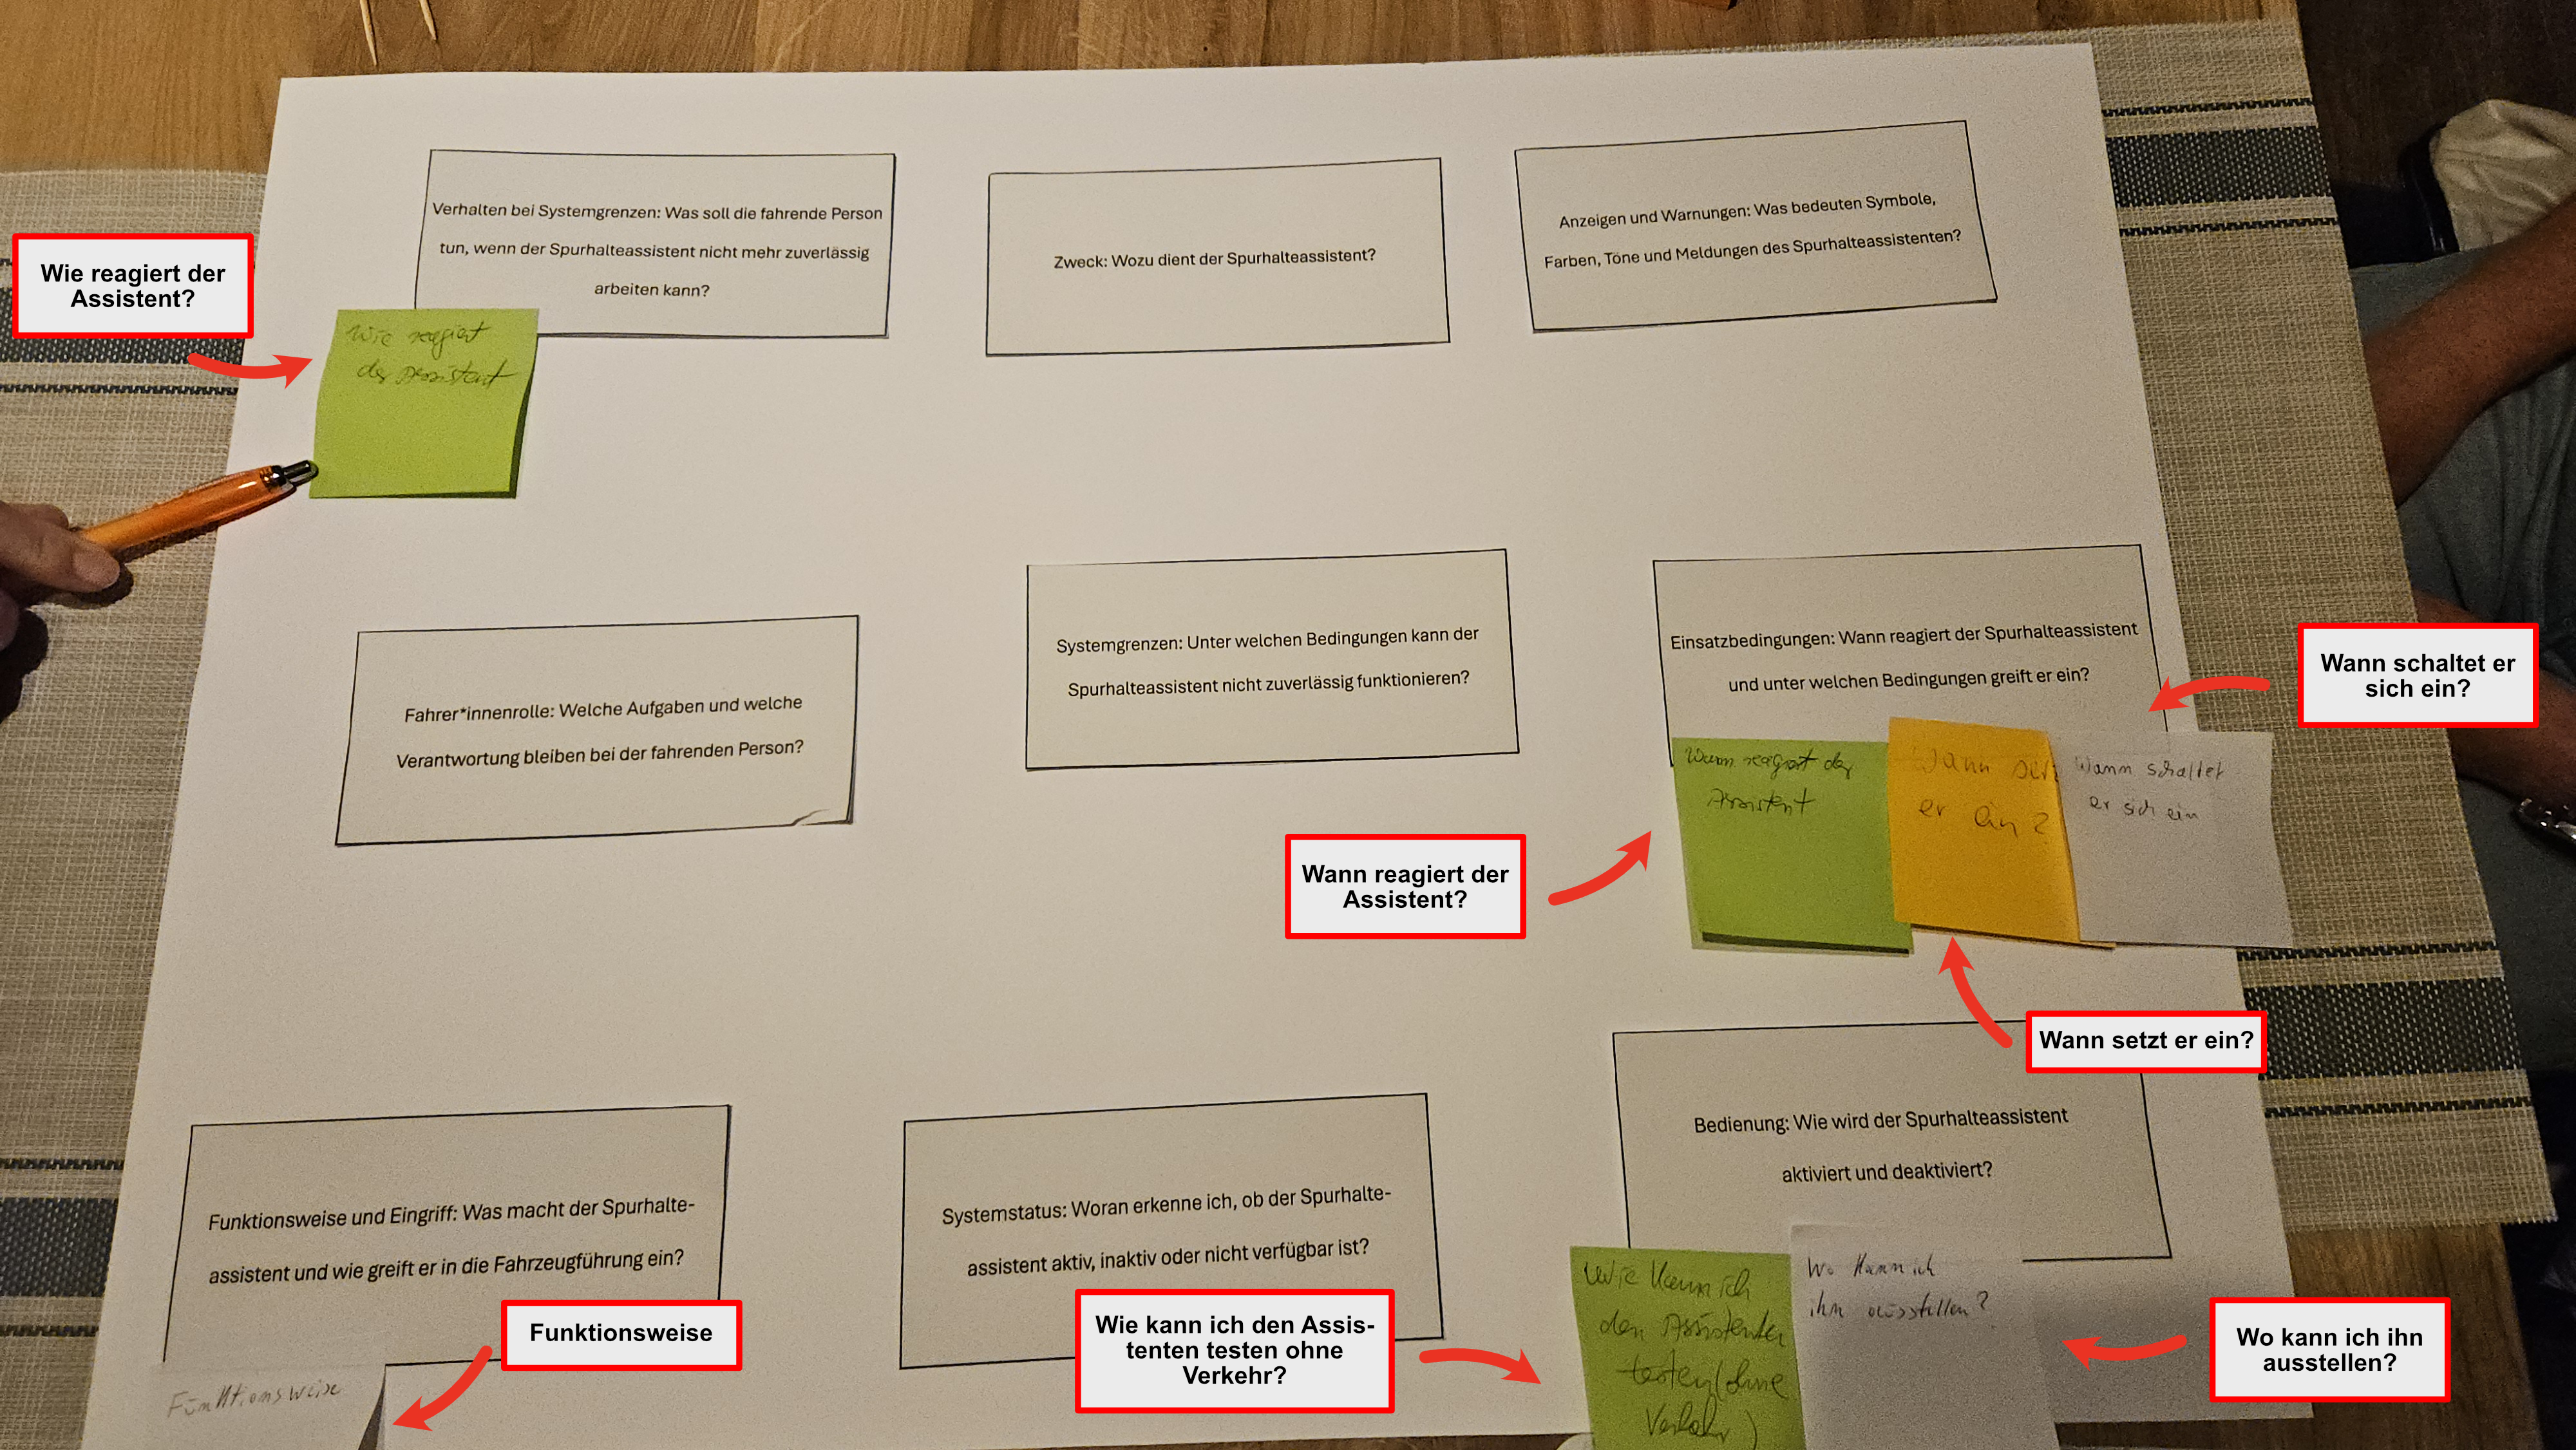
\includegraphics[width=0.9\textwidth]{images/results/Workshop_1/Ergebnisse_Collect.png}
    \caption{Ergebnisse der Collect-Phase des ersten Workshops}
    \label{fig:W1_Collect}
    \medskip
    {\footnotesize Quelle: Eigene Fotografie.}
\end{figure}

Die Teilnehmer*innen diskutierten ausführlich, unter welchen Bedingungen der Assistent eingreift, weswegen diese Themenkarte mit drei Post-its bedacht wurde. Das Post-it in der linken oberen Ecke der Abbildung kann auf den ersten Blick auch zu dieser Themenkarte gezählt werden, allerdings wollten die Teilnehmer*innen zum Ausdruck bringen, wie der Spurhalteassistent sich in einer Grenzsituation im Zusammenspiel mit der fahrzeugführenden Person verhält. Außerdem wurden Aktivierung und Deaktivierung neben der Funktionsweise als weitere Aspekte genannt. Viele Themenkarten erhielten von den Teilnehmer*innen keine Post-its und wurden auf Nachfrage nicht als zentral für die Fragestellung betrachtet.

Abbildung \ref{fig:W1_Choose_1} zeigt die Ergebnisse des Dot-Votings, welches eine Differenzierung nach persönicher Priorität ermöglicht. Eine besonders hohe Bedeutung wurde der Aktivierung und Deaktivierung des Assistenten beigemessen, was sich in der Anzahl der Klebepunkte (7 Punkte) wiederspiegelt. Außerdem schien einigen Teilnehmer*innen die Funktionsweise des Assistenten (3 Punkte) wichtig zu sein. 

\begin{figure}[H]
    \centering
    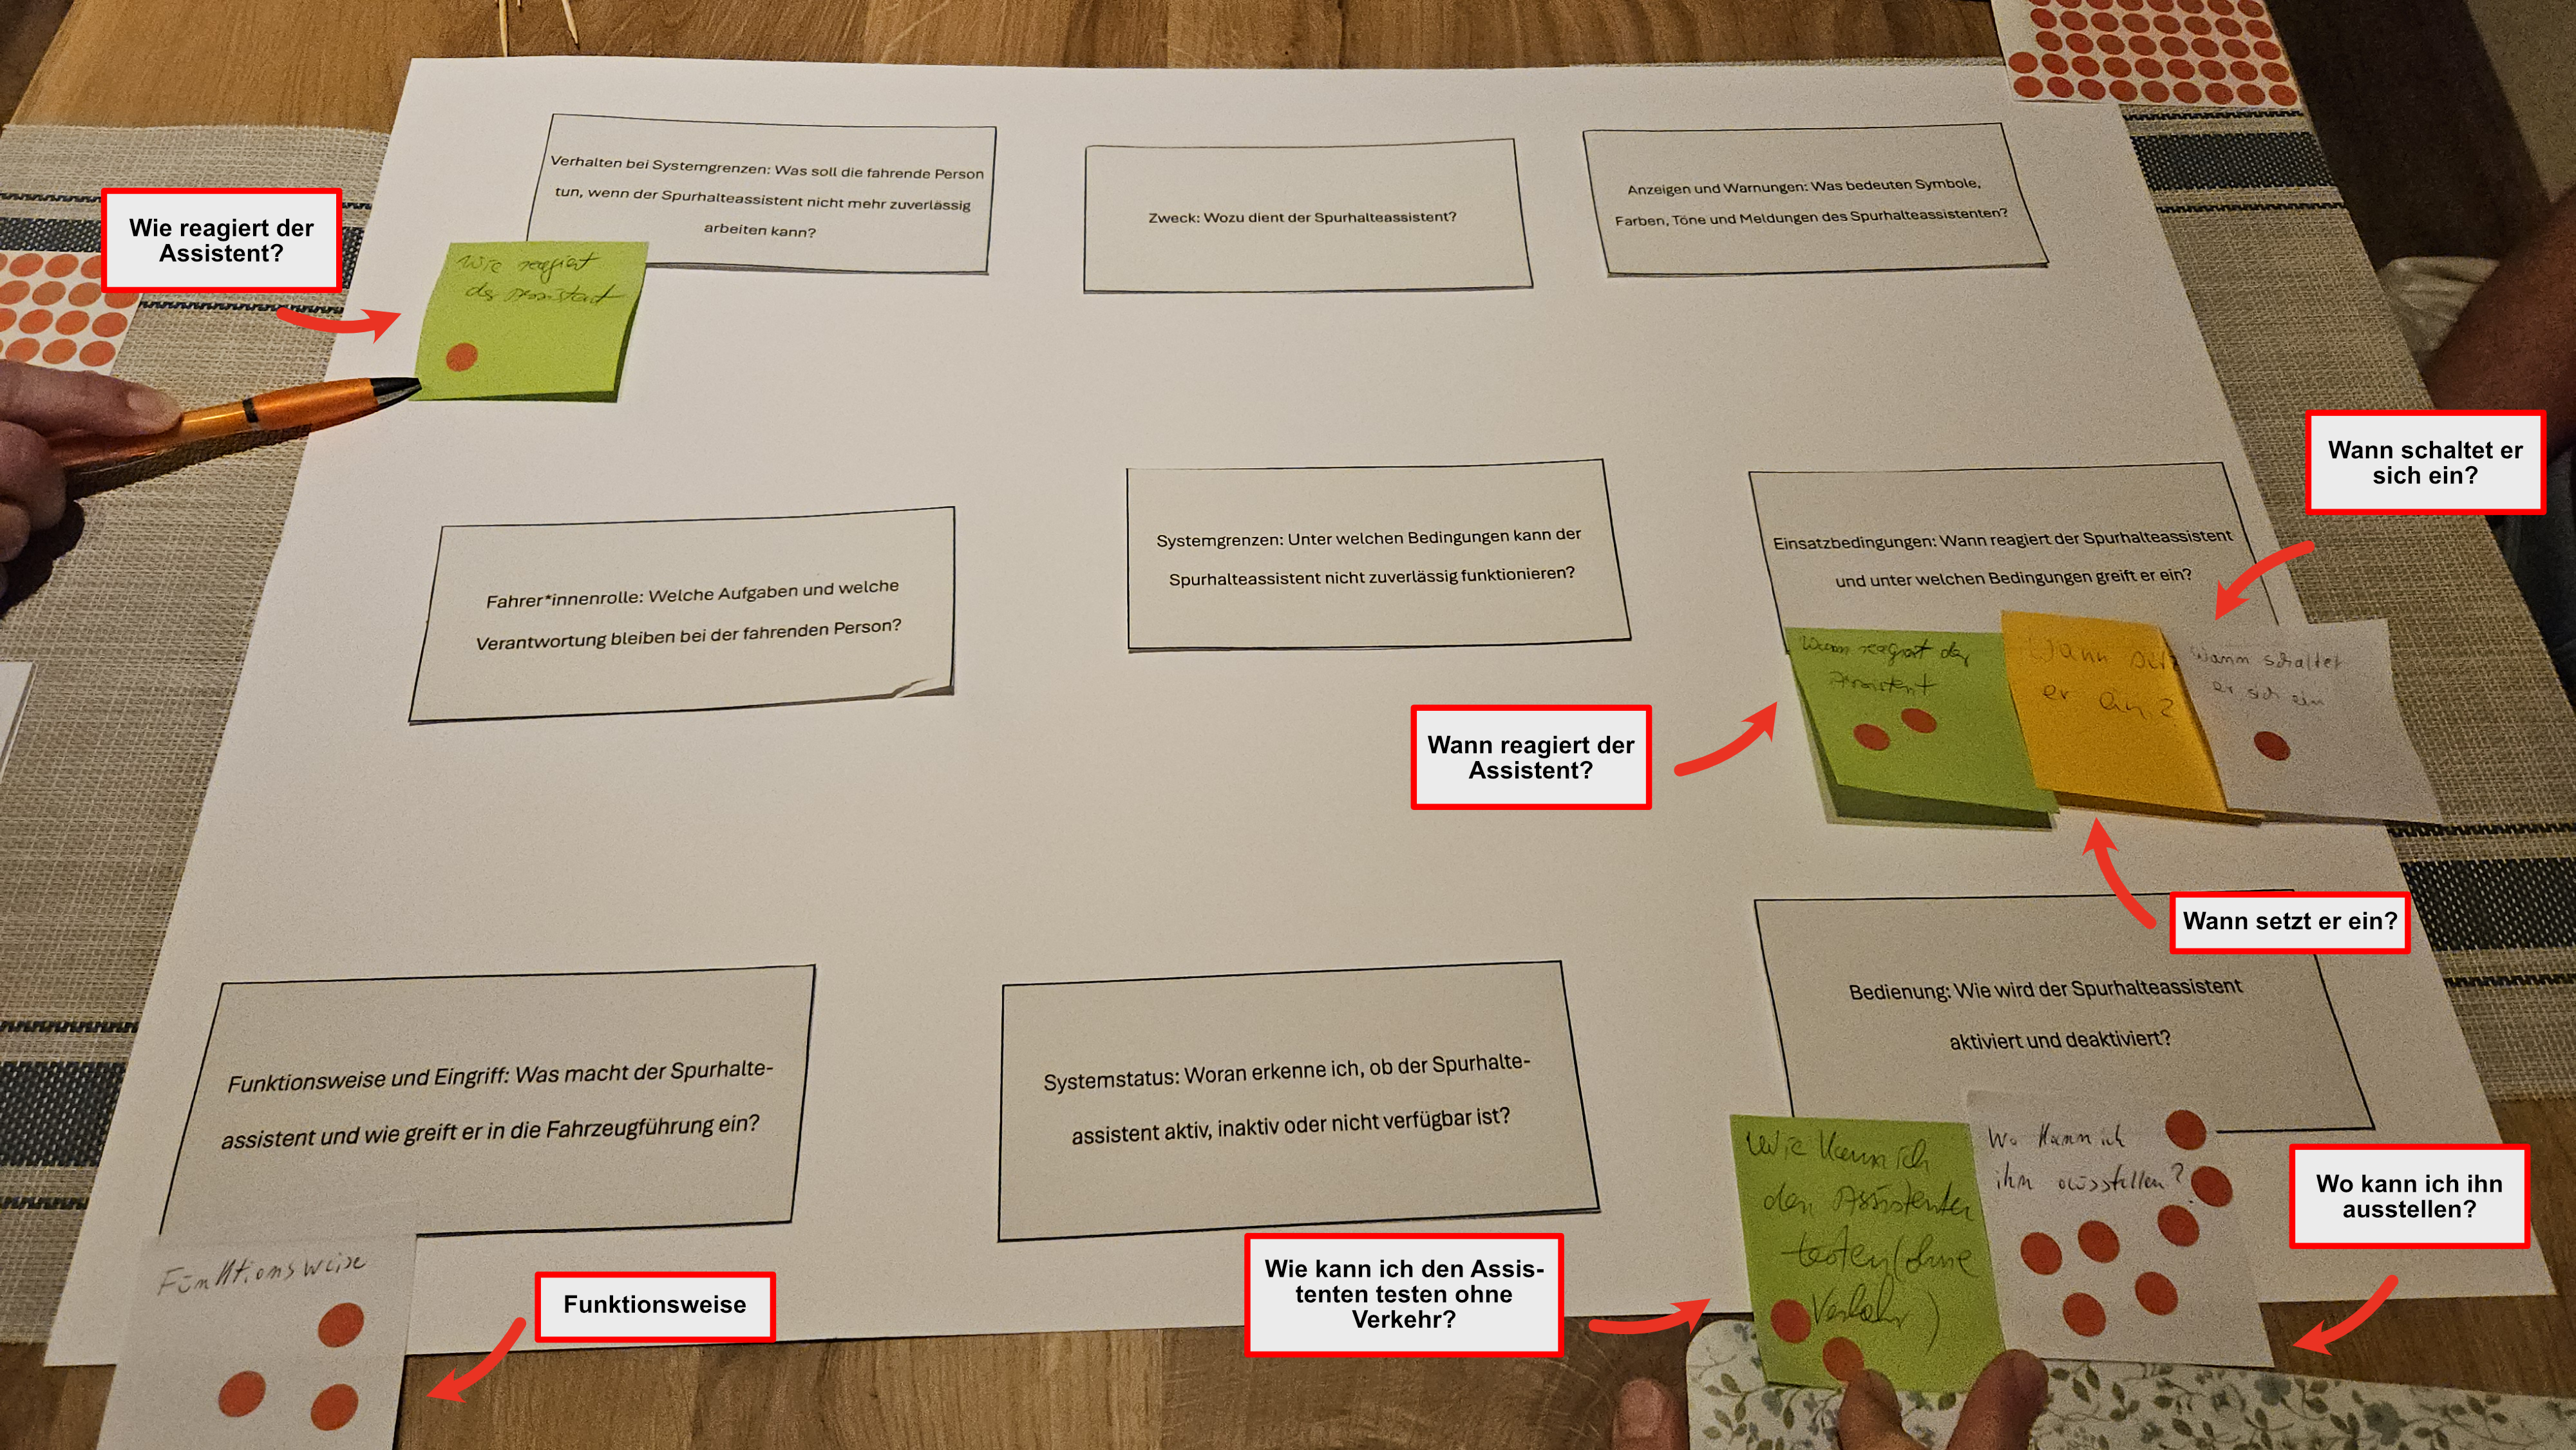
\includegraphics[width=0.9\textwidth]{images/results/Workshop_1/Ergebnisse_Choose_1.png}
    \caption{Ergebnisse der Choose-Phase des ersten Workshops}
    \label{fig:W1_Choose_1}
    \medskip
    {\footnotesize Quelle: Eigene Fotografie.}
\end{figure}

Abbildung \ref{fig:W1_Choose_2} zeigt die gemeinsame Ordnung der Post-its nach der Priorität für ein Onboarding.

\begin{figure}[H]
    \centering
    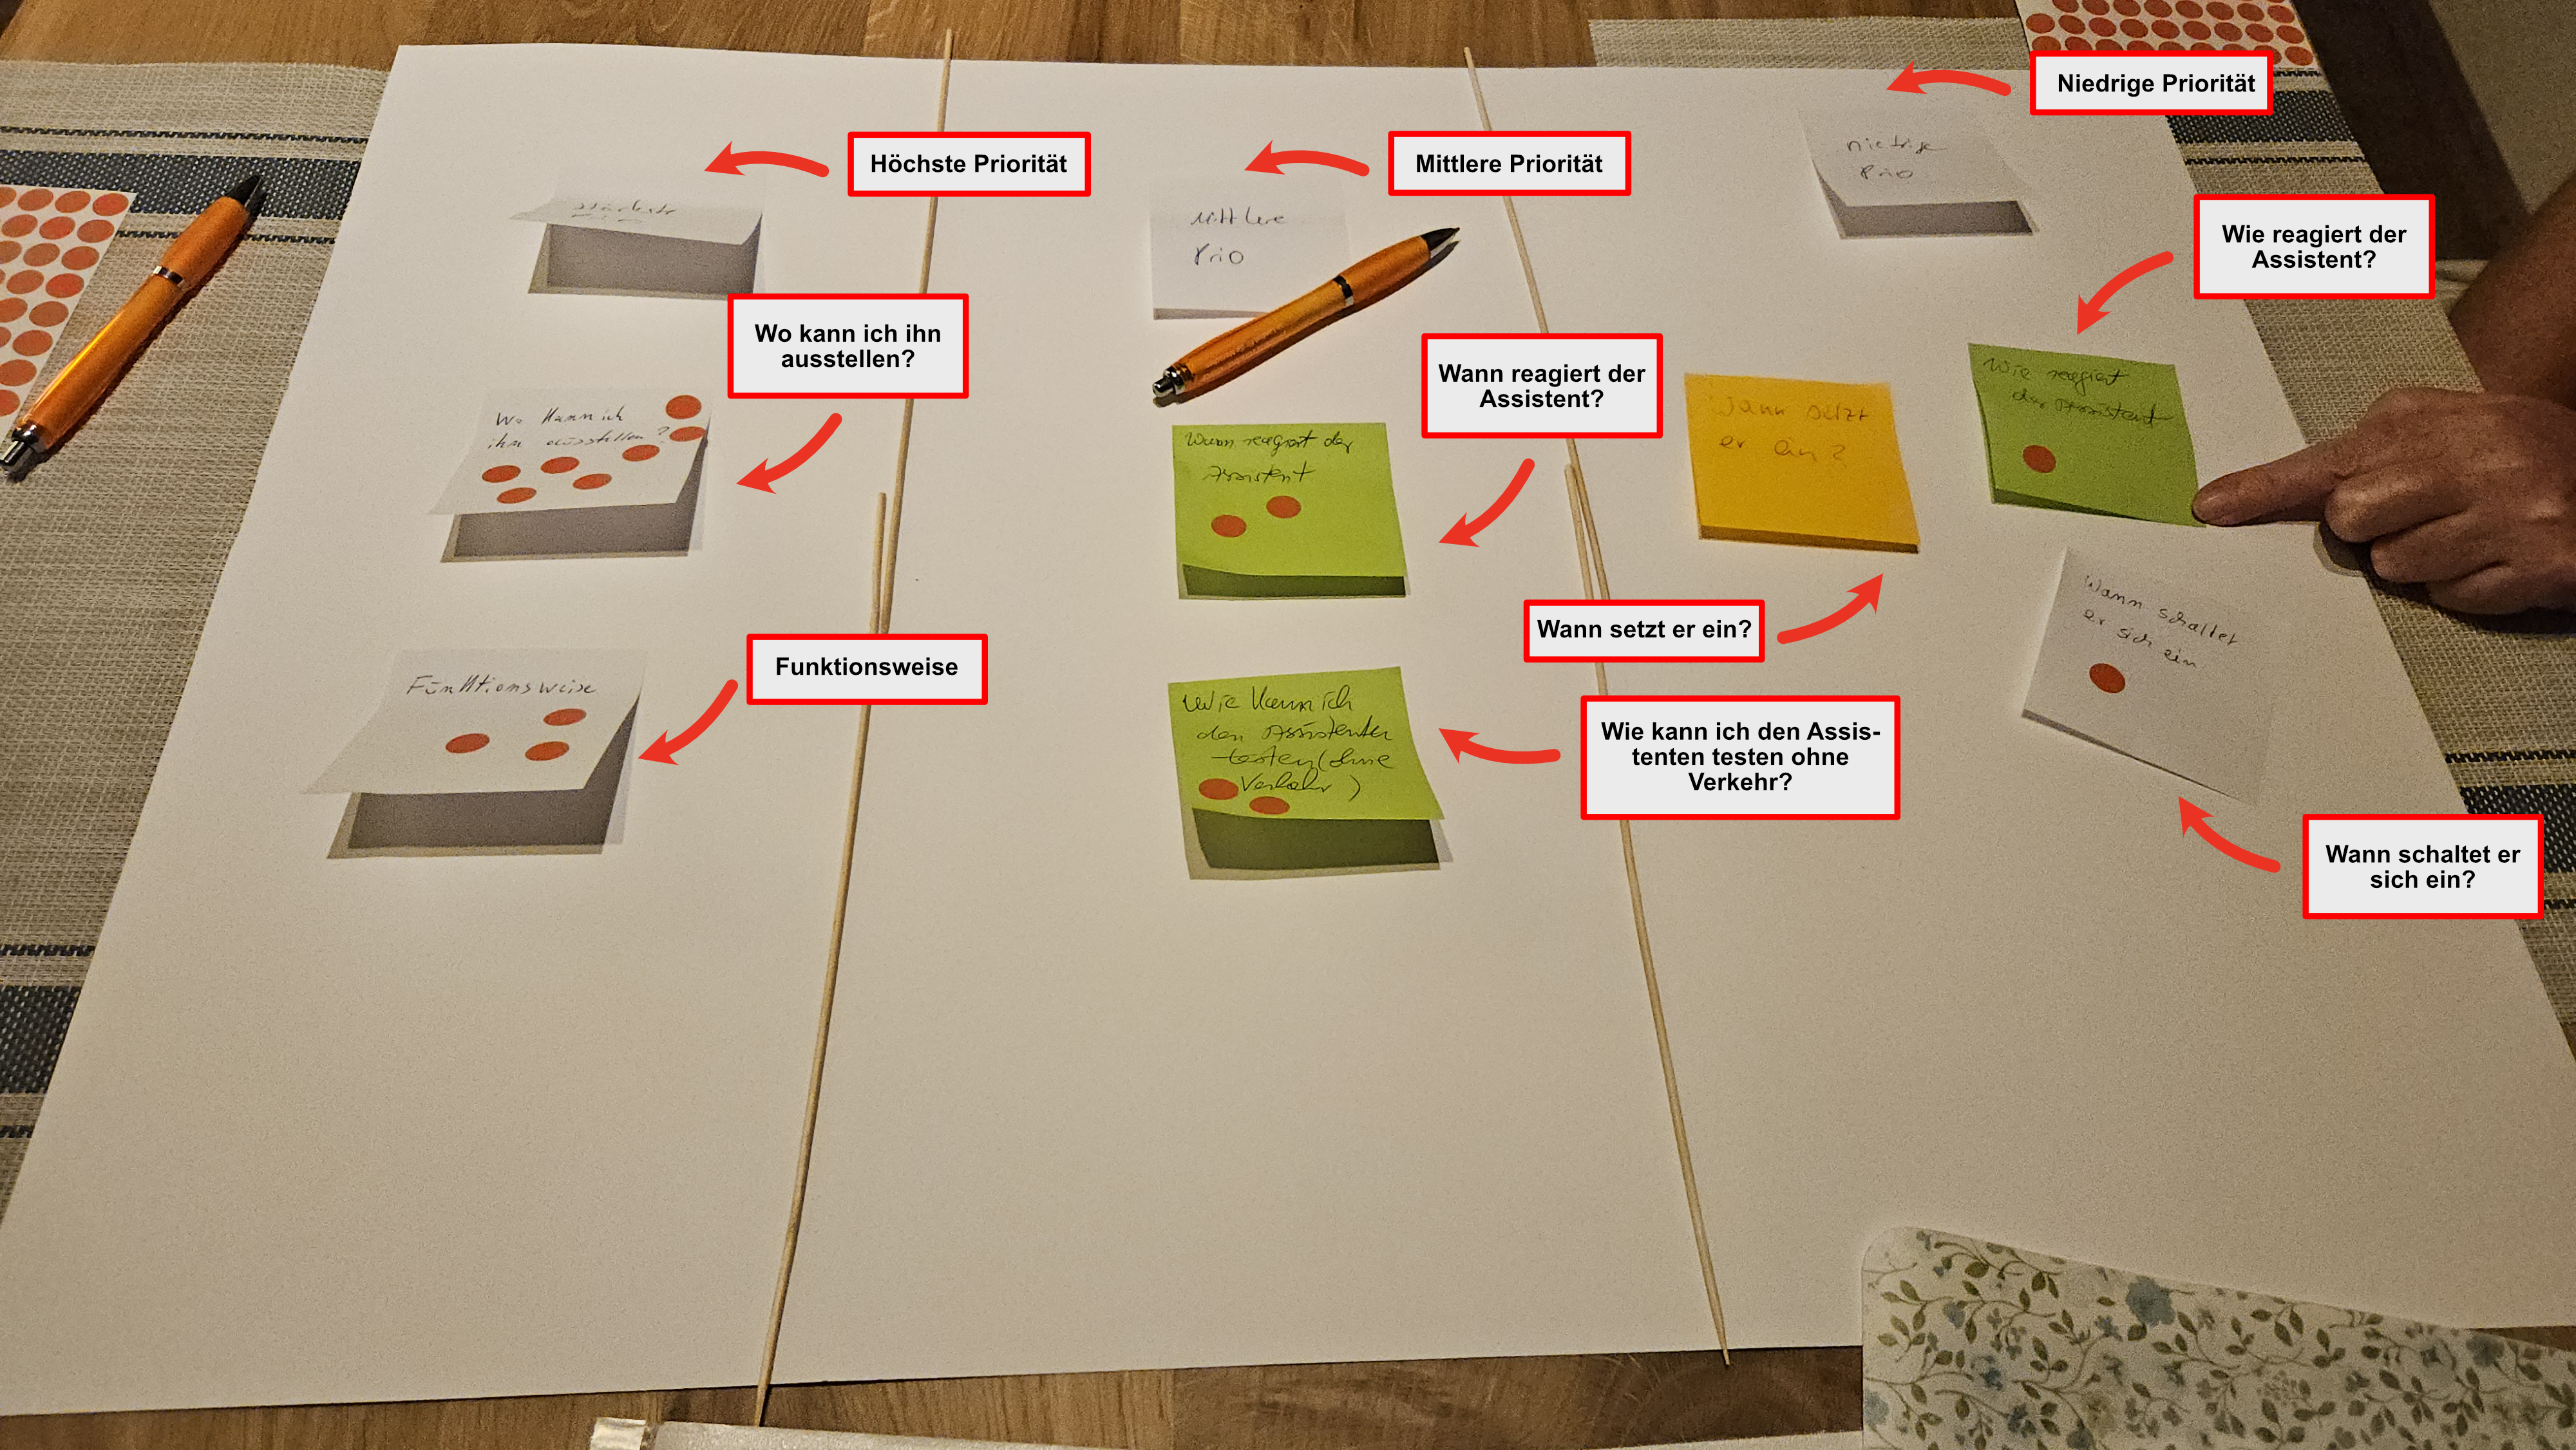
\includegraphics[width=0.9\textwidth]{images/results/Workshop_1/Ergebnisse_Choose_2.png}
    \caption{Ergebnisse der Choose-Phase des ersten Workshops}
    \label{fig:W1_Choose_2}
    \medskip
    {\footnotesize Quelle: Eigene Fotografie.}
\end{figure}

Es gab zwischen den Teilnehmer*innen keinen Dissenz bzgl. der Sortierung in die Matrix. Stattdessen nutzen sie die Klebepunkte als Indikator, um eine gemeinsame Ordnung festzulegen. Höchste Priorität hatten also auch hier die Aktivierung und Deaktivierung des Spurhalteassistenten sowie dessen Funktionsweise. Mit mittlerer Priorität wurden das Verhalten in Grenzsituationen und Tests außerhalb des Straßenverkehrs gekennzeichnet. Wann der Assistent selbst eingreift, hatte für die Teilnehmer*innen nur eine geringe Priorität.

Abbildung \ref{fig:W1_Choose_3} zeigt die im Anschluss durch die Teilnehmer*innen vorgenommene Unterteilung nach Informationszeitpunkten.

\begin{figure}[H]
    \centering
    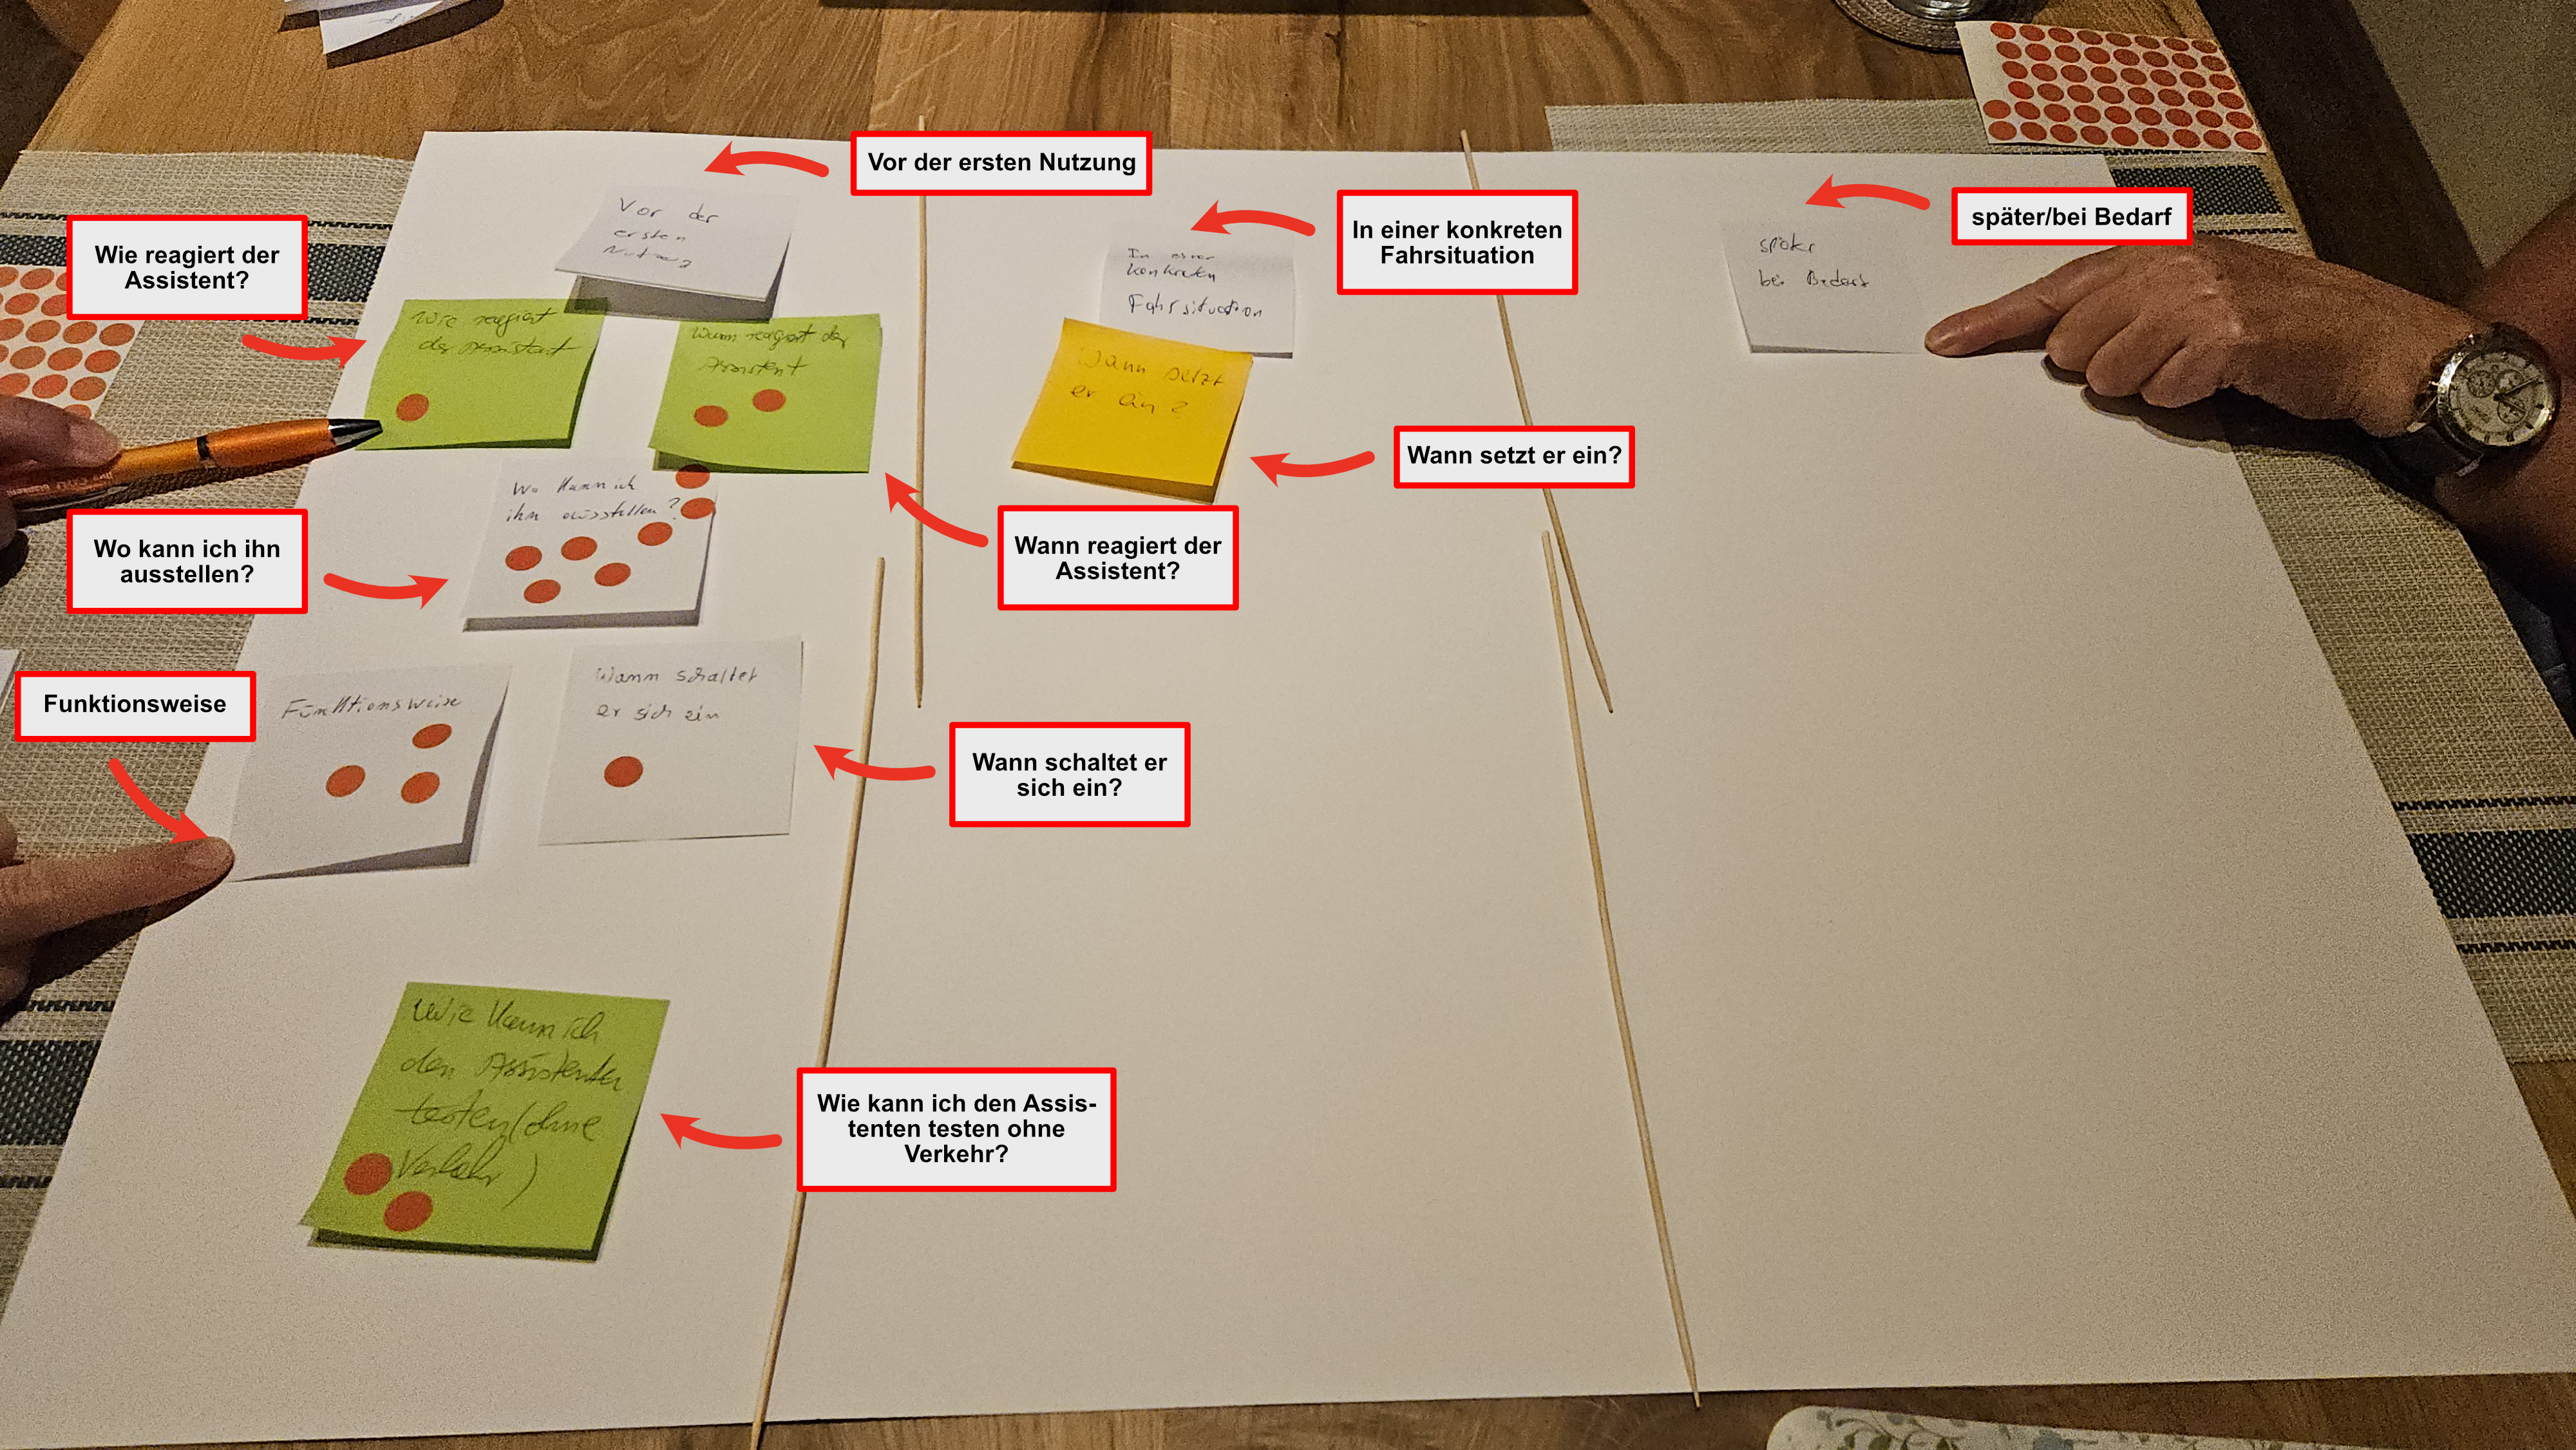
\includegraphics[width=0.9\textwidth]{images/results/Workshop_1/Ergebnisse_Choose_3.png}
    \caption{Ergebnisse der Choose-Phase des ersten Workshops}
    \label{fig:W1_Choose_3}
    \medskip
    {\footnotesize Quelle: Eigene Fotografie.}
\end{figure}

Auffällig ist, dass sich alle Post-its, welchen in den vorherigen Schritten anhand der Klebepunkte und der anschließenden Sortierung eine hohe Priorität beigemessen wurde, in der linken Spalte befinden. Die Proband*innen waren sich einig, dass diese Aspekte vor Fahrtantritt vermittelt werden müssen. Der Spalte 'In einer konkreten Fahrsituation' wurde nur ein einziger Post-it zugewiesen, welchem zuvor eine niedrige Priorität attestiert wurde. Später oder bei Bedarf wurde kein Post-it zugewiesen.

Zuletzt soll noch die Ergebnisübersicht der Create-Phase getrennt nach den beiden Szenarien gezeigt werden. Abbildung \ref{fig:W1_Commit} zeigt diese Übersicht. Eine vergrößerte Darstellung der einzelnen Entwürfe lässt sich in Anhang \ref{sec:gestaltungslösungen_w1} finden. Die Abbildung soll an dieser Stelle zeigen, dass die Proband*innen für das Szenario A vor Fahrtantritt, entsprechend ihrer zuvor geäußerten Präferenzen für den Informationszeitpunkt, deutlich mehr Materialien nutzten, als für das Szenario B in einer konkreten Fahrsituation. Dennoch erhielt einer der Entwürfe auf der rechten Seite im anschließenden Dot-Voting bzgl. der für die Teilnehmer*innen besonders wichtigen Gestaltungselemente die meisten Stimmen. 

\begin{figure}[H]
    \centering
    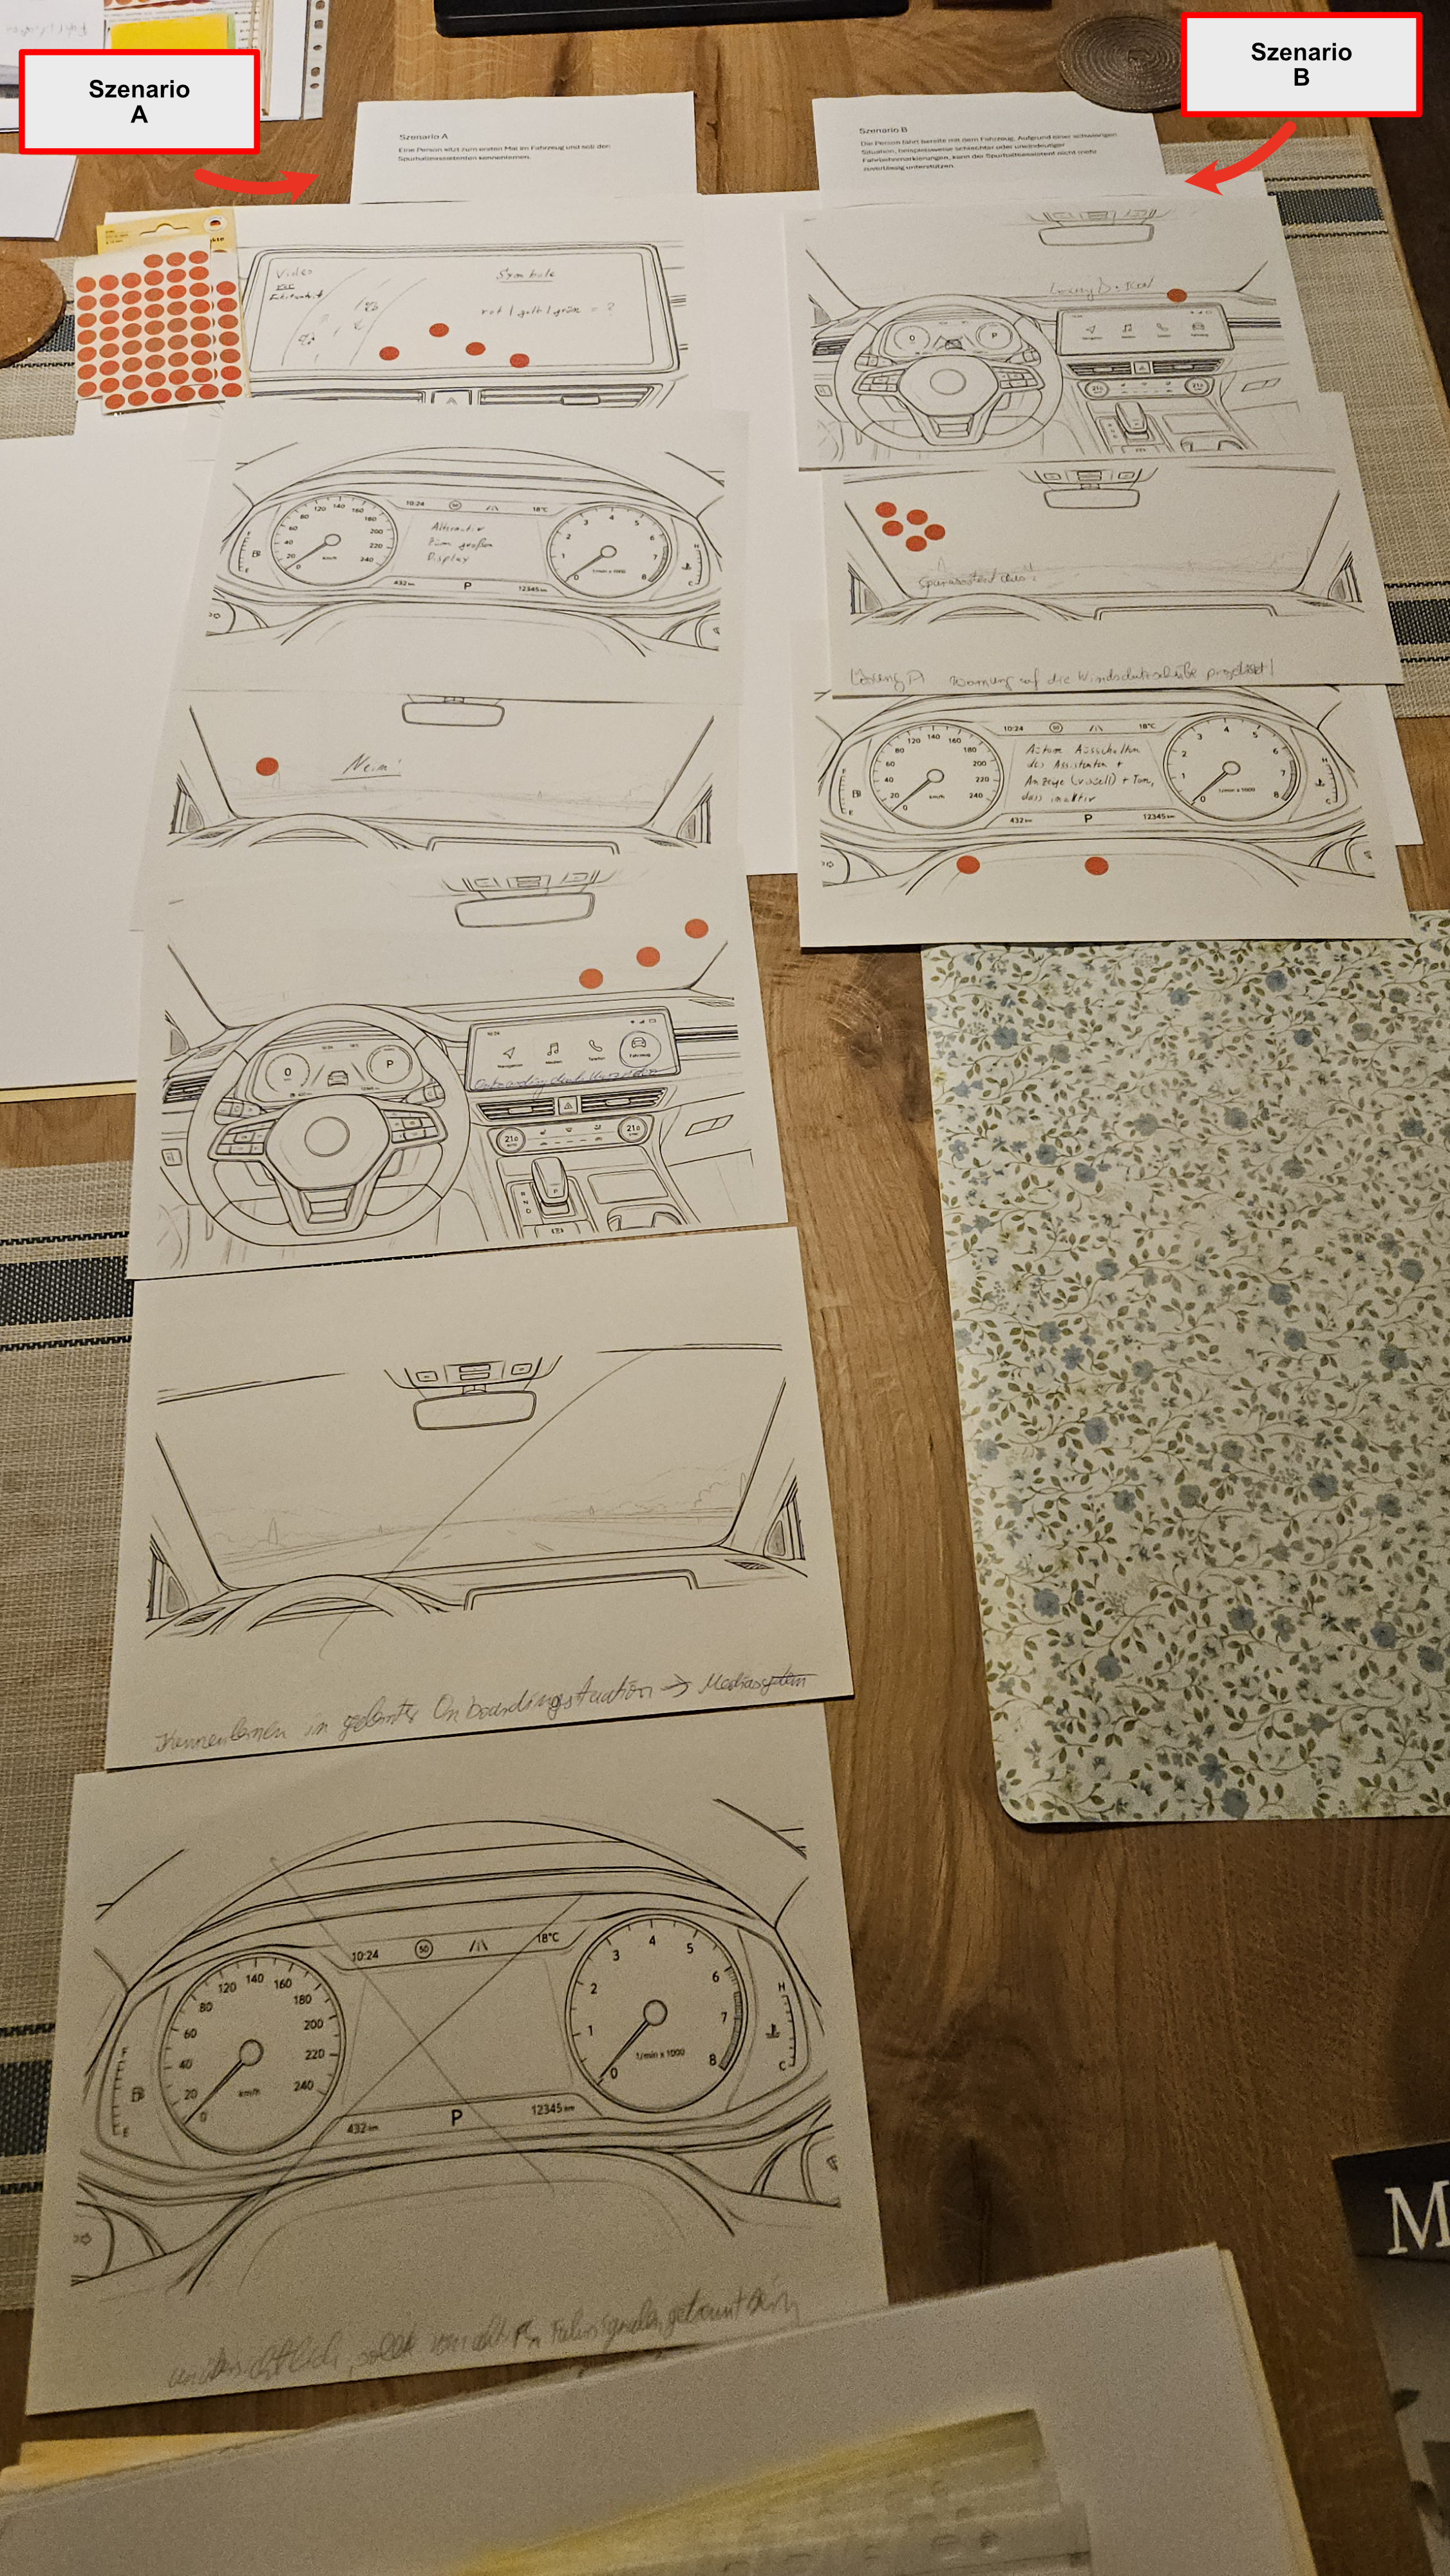
\includegraphics[width=1\textwidth,height=0.95\textheight,keepaspectratio]{images/results/Workshop_1/Ergebnisse_Commit.png}
    \caption{Ergebnisse der Commit-Phase des ersten Workshops}
    \label{fig:W1_Commit}
    \medskip
    {\footnotesize Quelle: Eigene Fotografie.}
\end{figure}

\subsubsection{Workshop zwei}
\label{subsubsec:Ergebnisse_Workshop_zwei}

Abbildung \ref{fig:W1_Collect} zeigt die Ergebnisse der Collect-Phase des zweiten Workshops.

\begin{figure}[H]
    \centering
    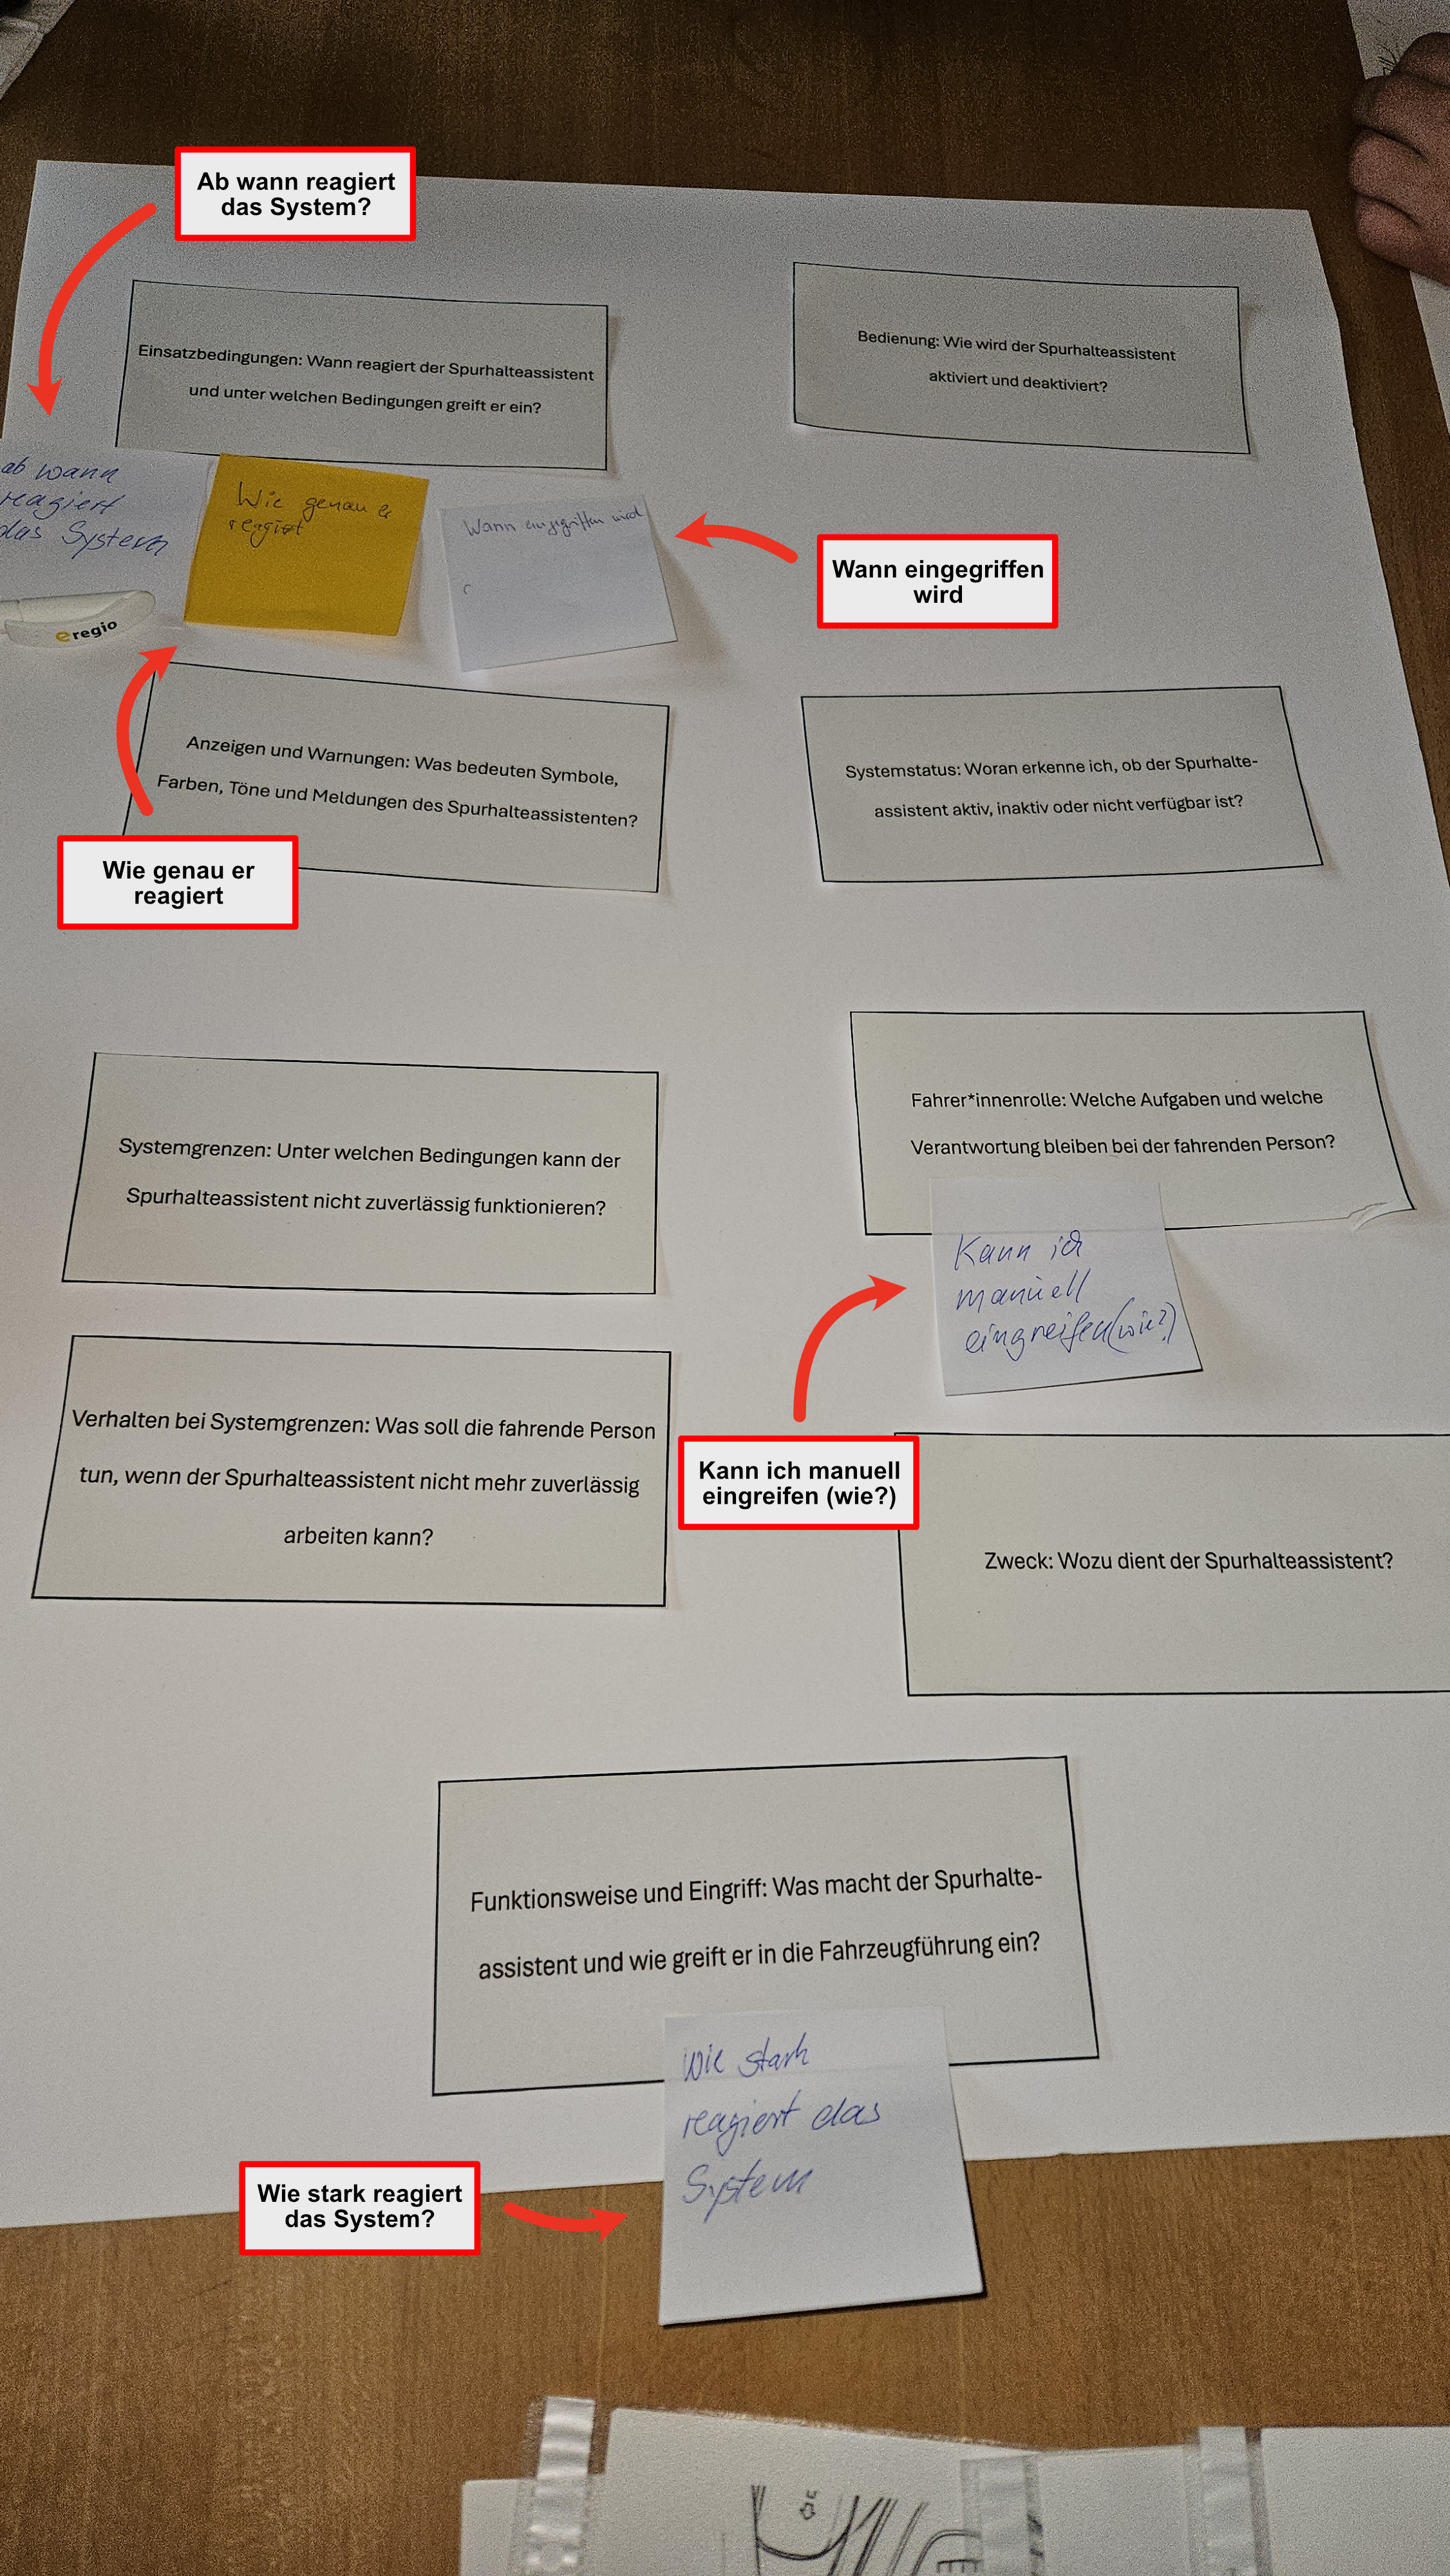
\includegraphics[width=0.65\textwidth]{images/results/Workshop_2/Ergebnisse_Collect.png}
    \caption{Ergebnisse der Collect-Phase des zweiten Workshops}
    \label{fig:W2_Collect}
    \medskip
    {\footnotesize Quelle: Eigene Fotografie.}
\end{figure}

Es lässt sich anhand der Menge der Post-its ein erster Interessenschwerpunkt in der linken oberen Ecke erkennen. Demnach lässt sich eine hohe Schnittmenge zum ersten Workshop feststellen, in dem ebenfalls die Themenkarte zu den Einsatzbedingungen des Spurhalteassistenten mit den meisten Post-its ausgestattet wurde. Auch bzgl. Funktionsweise und Eingriff (unterer Bildrand) lassen sich Gemeinsamkeiten zwischen den Workshops erkennen. Im Unterschied zum ersten Workshop gab es auch ein Post-it zur Rolle der Fahrer*innen, da für eine Person wichtig erschien, wie man manuell in das Fahrgeschehen eingreifen könne.

\clearpage

Abbildung \ref{fig:W2_Choose_1} zeigt das Ergebnis des anschließenden Dot-Votings.

\begin{figure}[H]
    \centering
    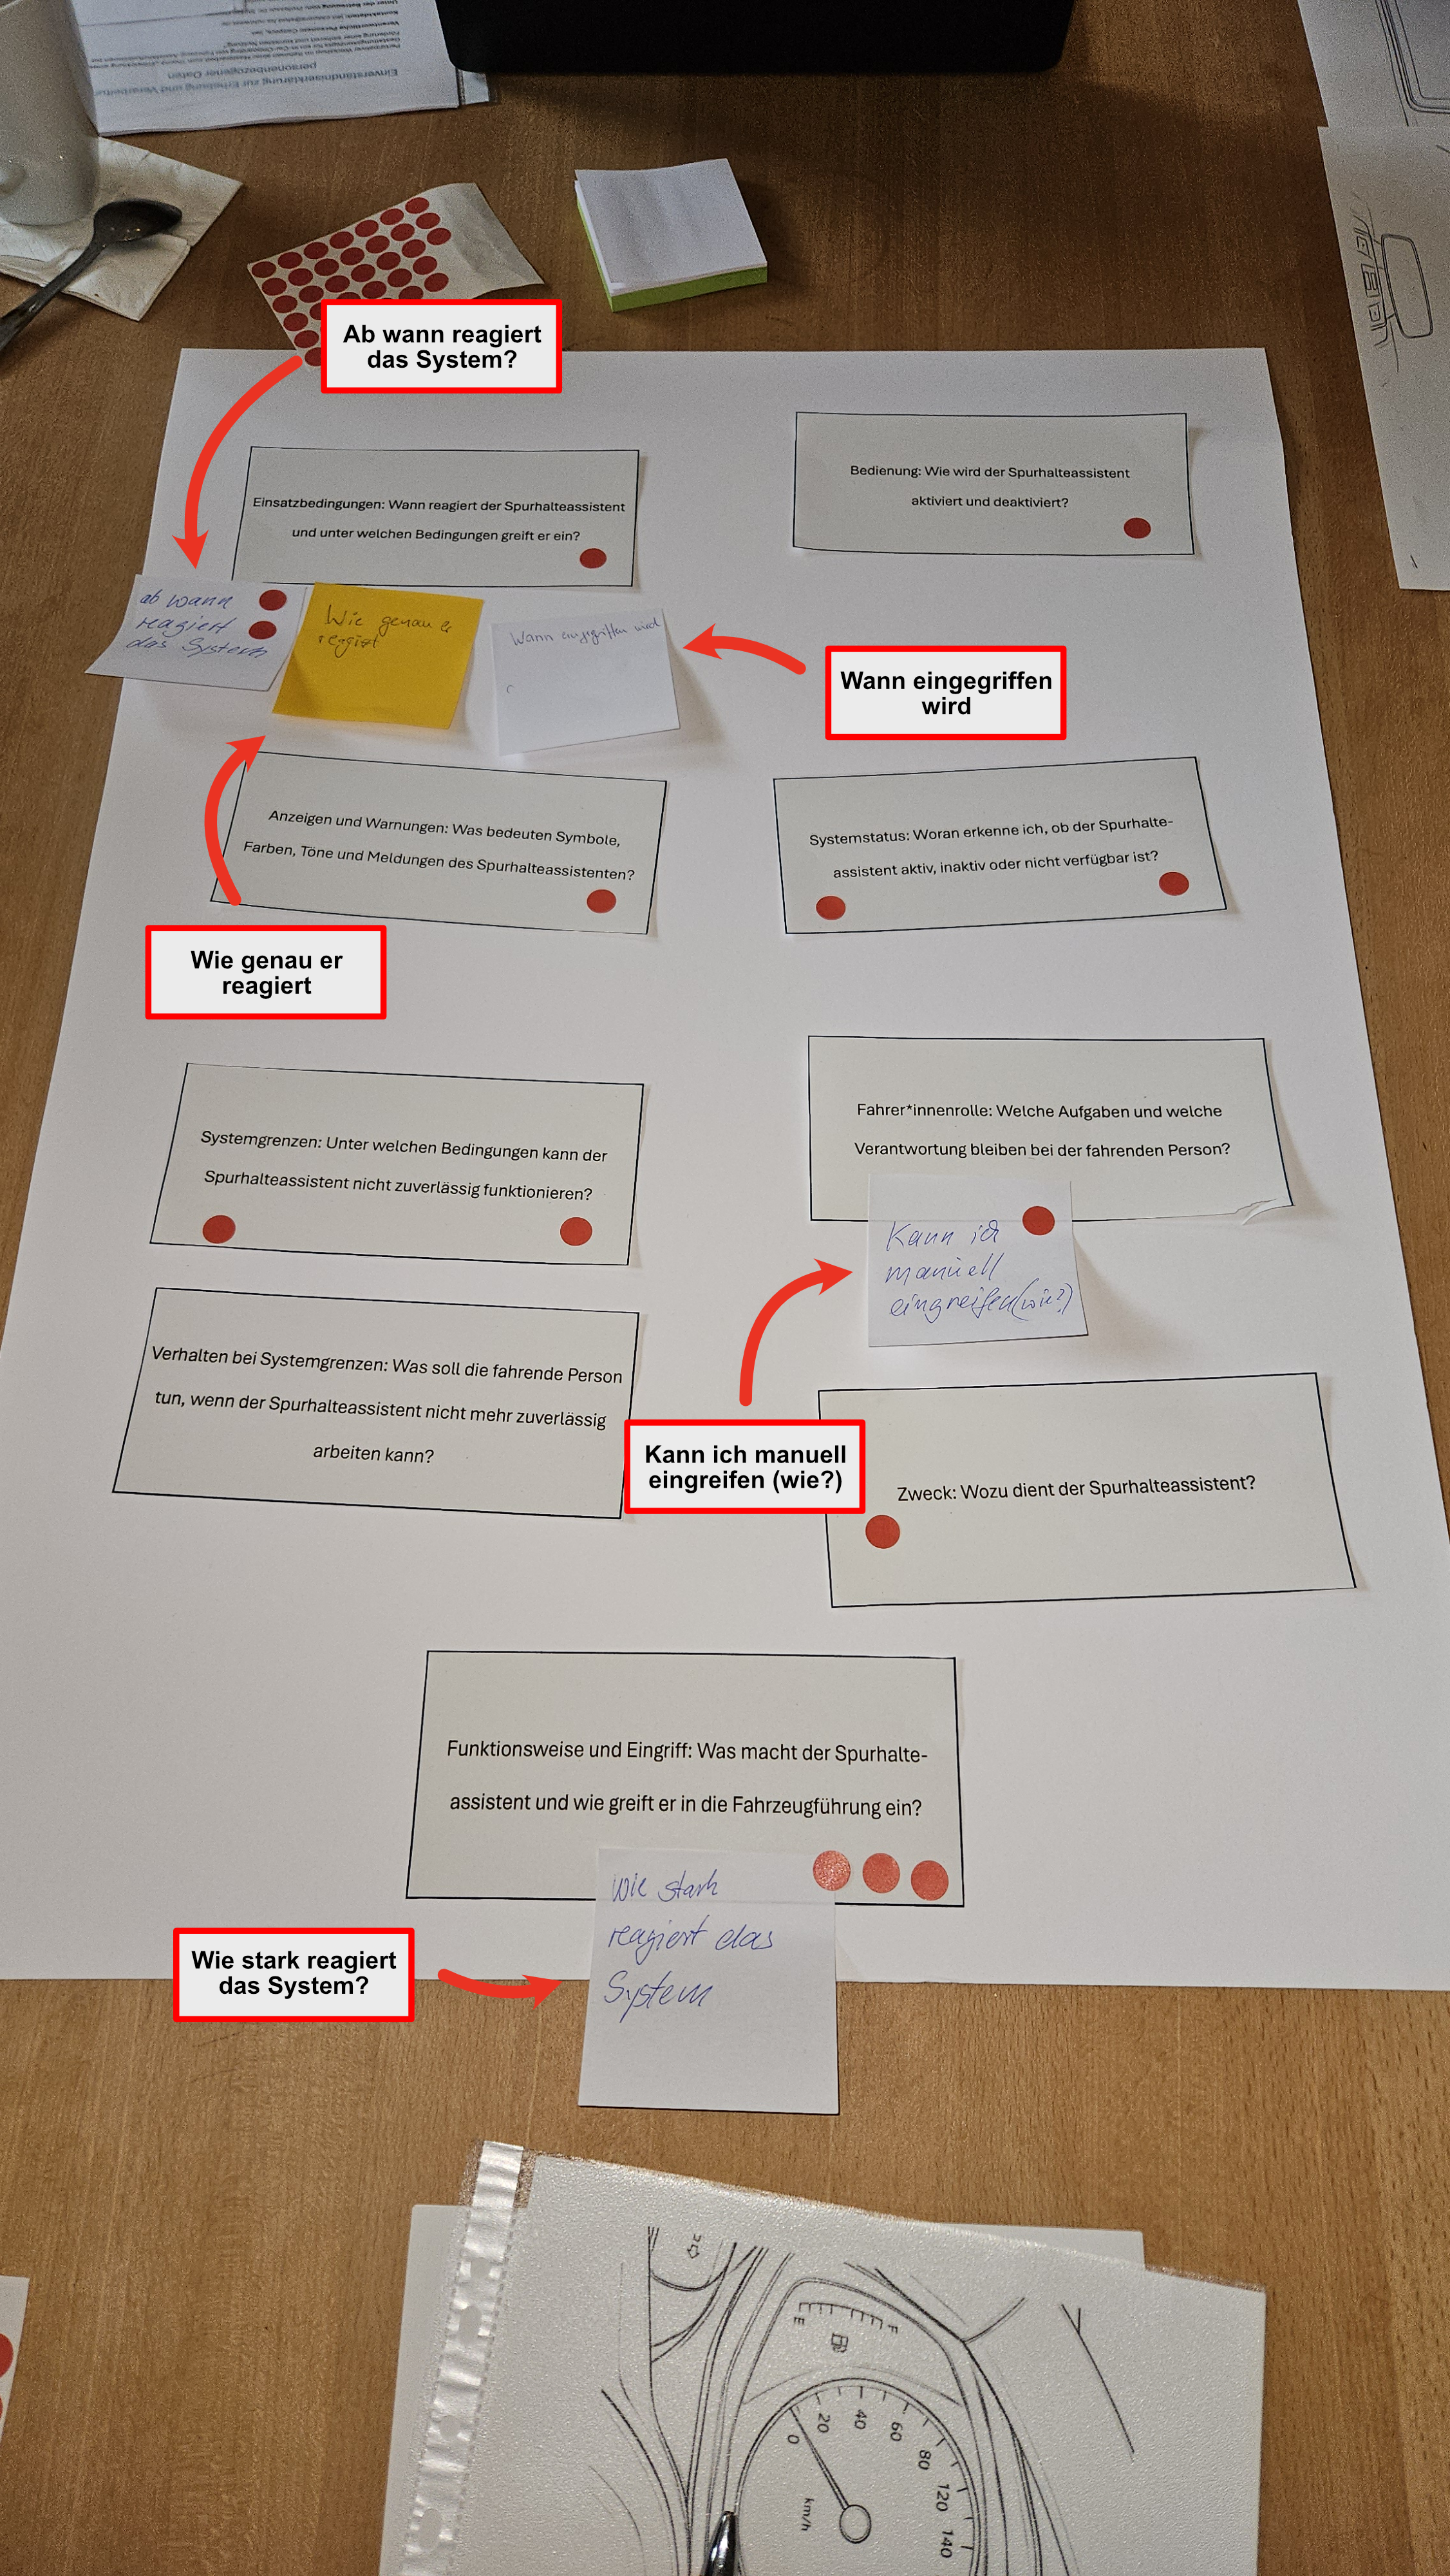
\includegraphics[width=0.65\textwidth]{images/results/Workshop_2/Ergebnisse_Choose_1.png}
    \caption{Ergebnisse der Choose-Phase des zweiten Workshops}
    \label{fig:W2_Choose_1}
    \medskip
    {\footnotesize Quelle: Eigene Fotografie.}
\end{figure}

Im Unterschied zum ersten Workshop, haben die Teilnehmer*innen, so wie es der Leitfaden eigentlich vorsah, nicht nur über die von ihnen angefertigten Post-its abgestimmt. Nachdem die Moderation den Teilnehmer*innen mögliche Themenkarten zur Gliederung präsentierte, äußerten einige Personen den Wunsch, auch über Aspekte abstimmen zu dürfen, welche nicht ihren eigenen Gedankengängen entstammten (Themenkarten ohne Post-its). Dies begründeten sie mit der aus ihrer Sicht gegebenen inhaltlichen Relevanz. Die Moderation traf die Entscheidung dem Wunsch zu entsprechen, da die anschließende Priorisierung dennoch von den Teilnehmer*innen ausging und dies auch im ersten Workshop möglich gewesen wäre. Dies führte schlussendlich dazu, dass die Klebepunkte, im Vergleich zum ersten Workshop, stärker über die Themenkarten verteilt wurden. Die meisten Stimmen erhielten die Themenkarten 'Funktionsweise und Eingriff' sowie Einsatzbedingungen.

\clearpage

Abbildung \ref{fig:W2_Choose_2} zeigt die Ergebnisse der anschließenden Priorisierung.

\begin{figure}[H]
    \centering
    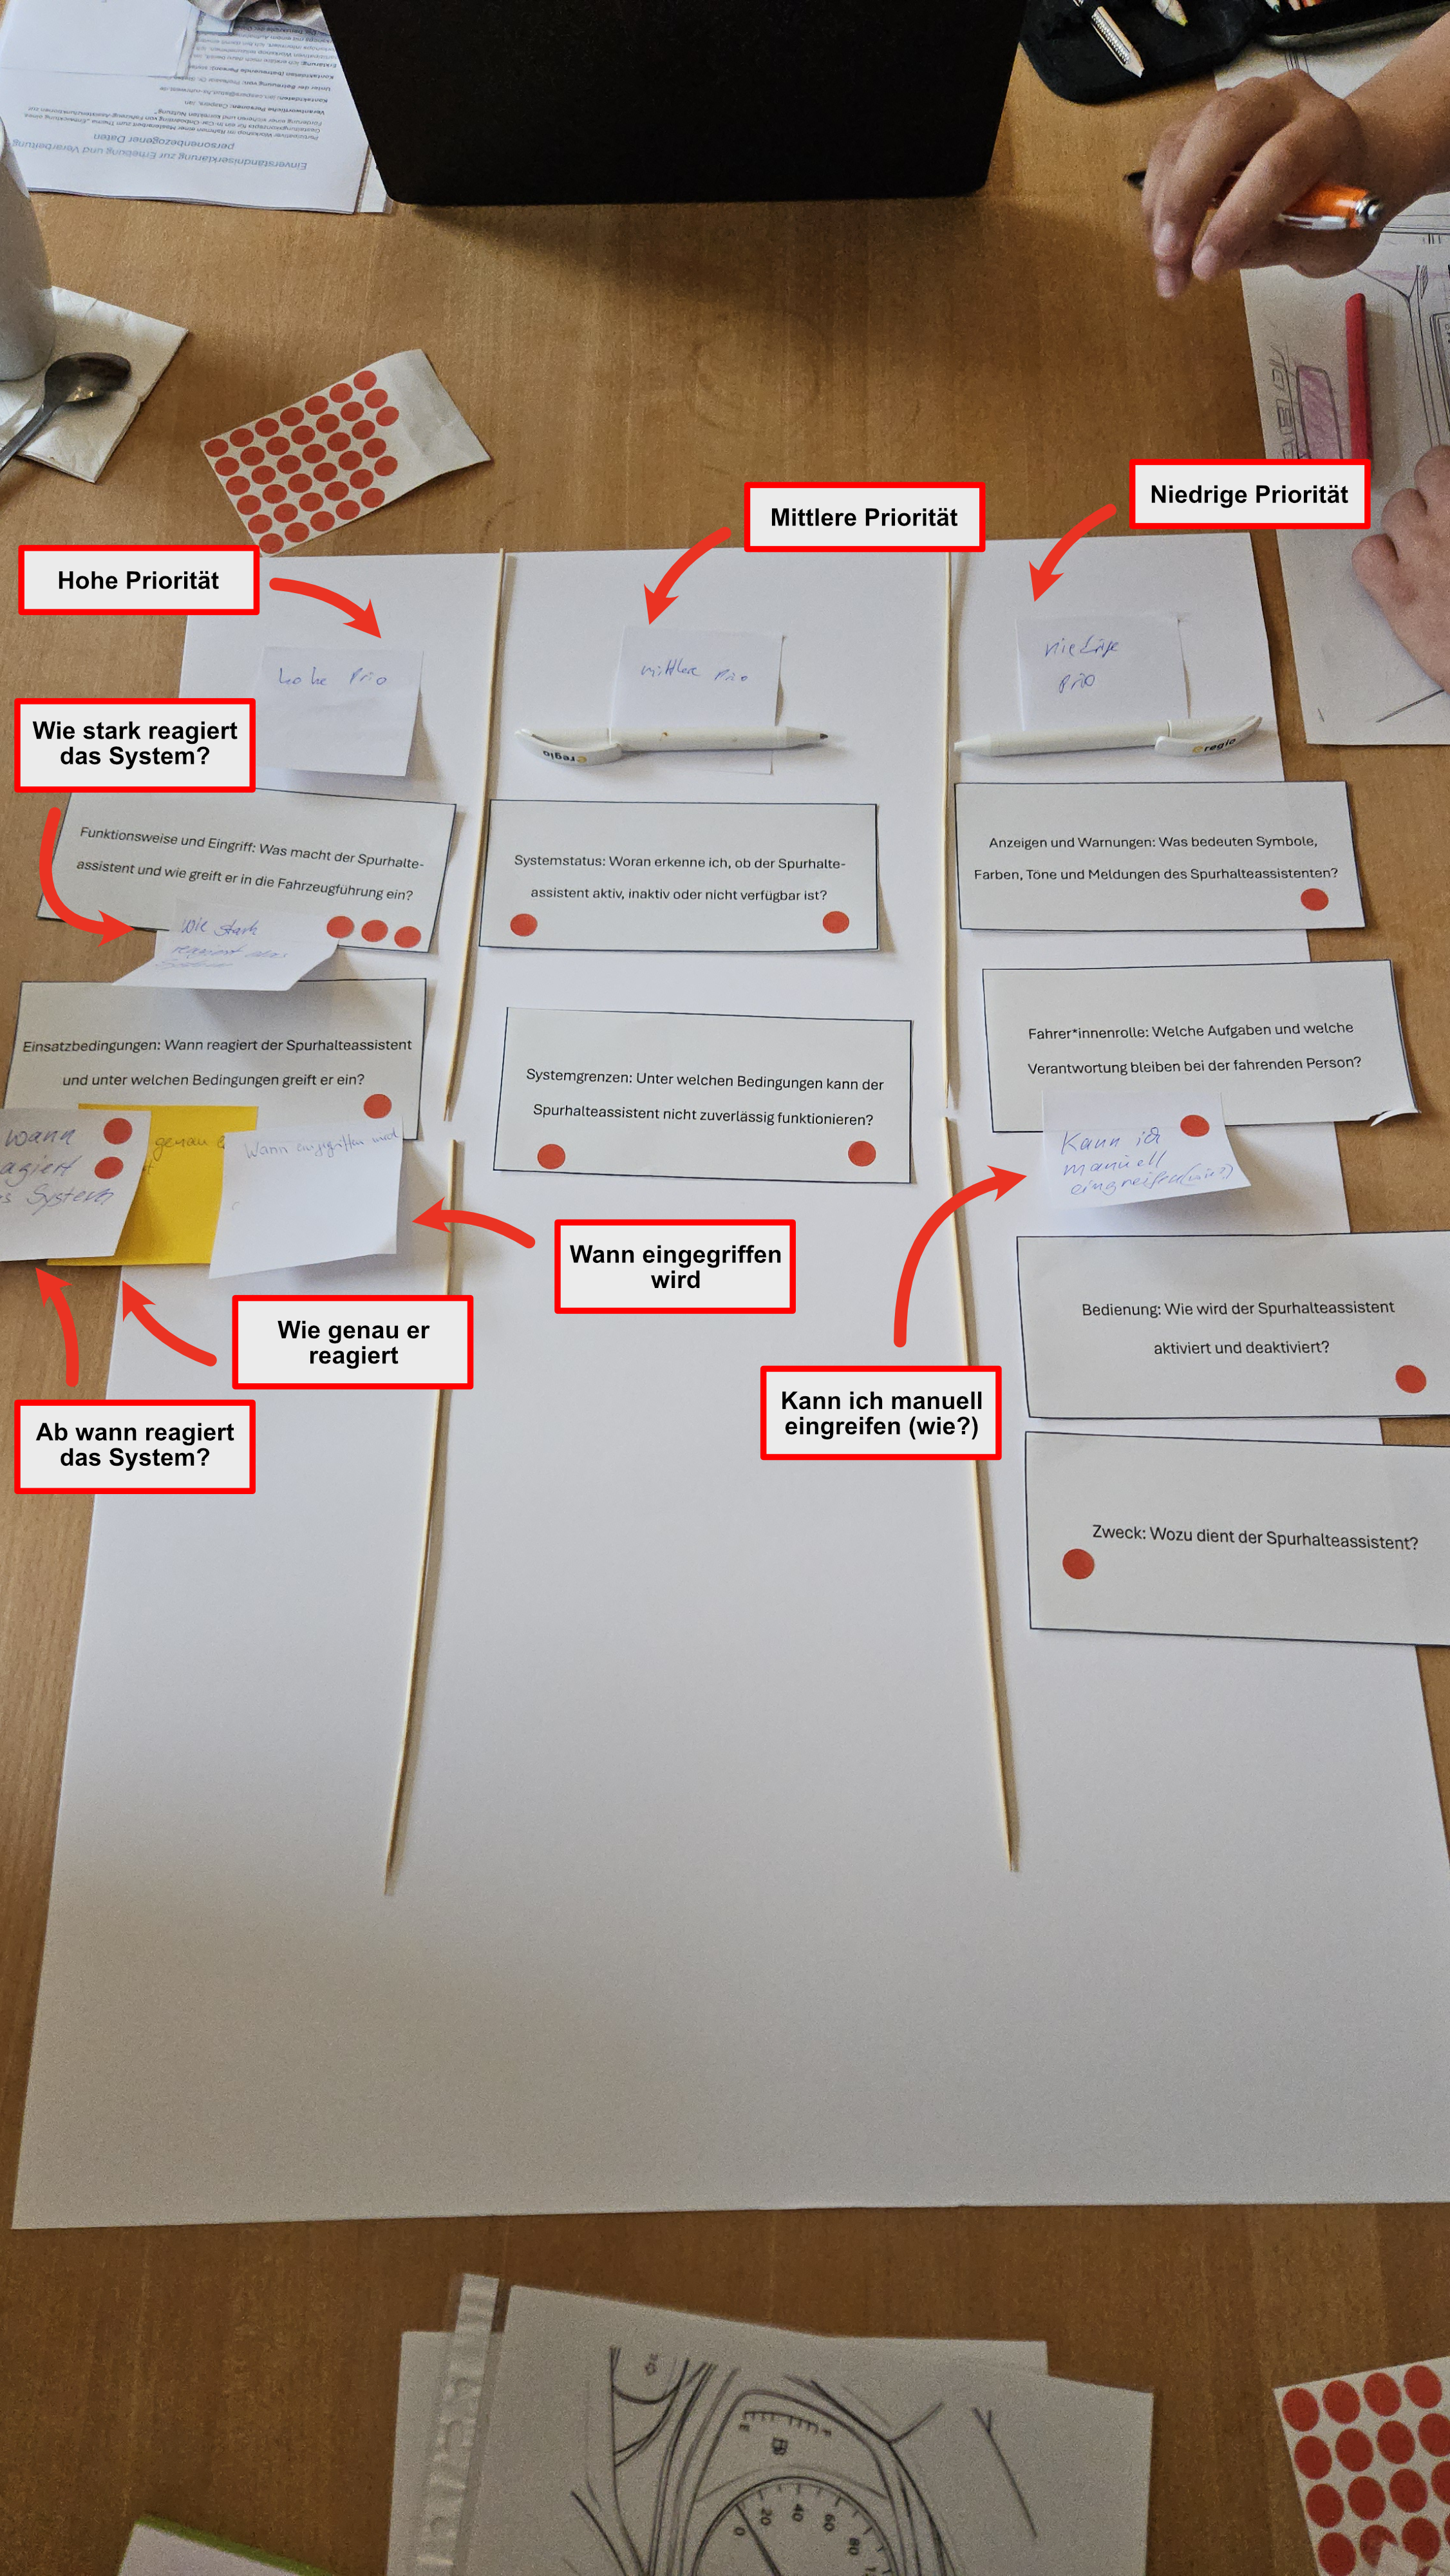
\includegraphics[width=0.65\textwidth]{images/results/Workshop_2/Ergebnisse_Choose_2.png}
    \caption{Ergebnisse der Choose-Phase des zweiten Workshops}
    \label{fig:W2_Choose_2}
    \medskip
    {\footnotesize Quelle: Eigene Fotografie.}
\end{figure}

Die Teilnehmer*innen orientierten sich nach eigener Aussage an den verteilten Klebepunkten und konnten sich schnell auf ein gemeinsames Ergebnis einigen, weswegen die einzelnen Post-its und Themenkarten an dieser Stelle nicht erneut vorgestellt werden müssen.

\clearpage

Abbildung \ref{fig:W2_Choose_3} zeigt die Unterteilung nach Informationszeitpunkten.

\begin{figure}[H]
    \centering
    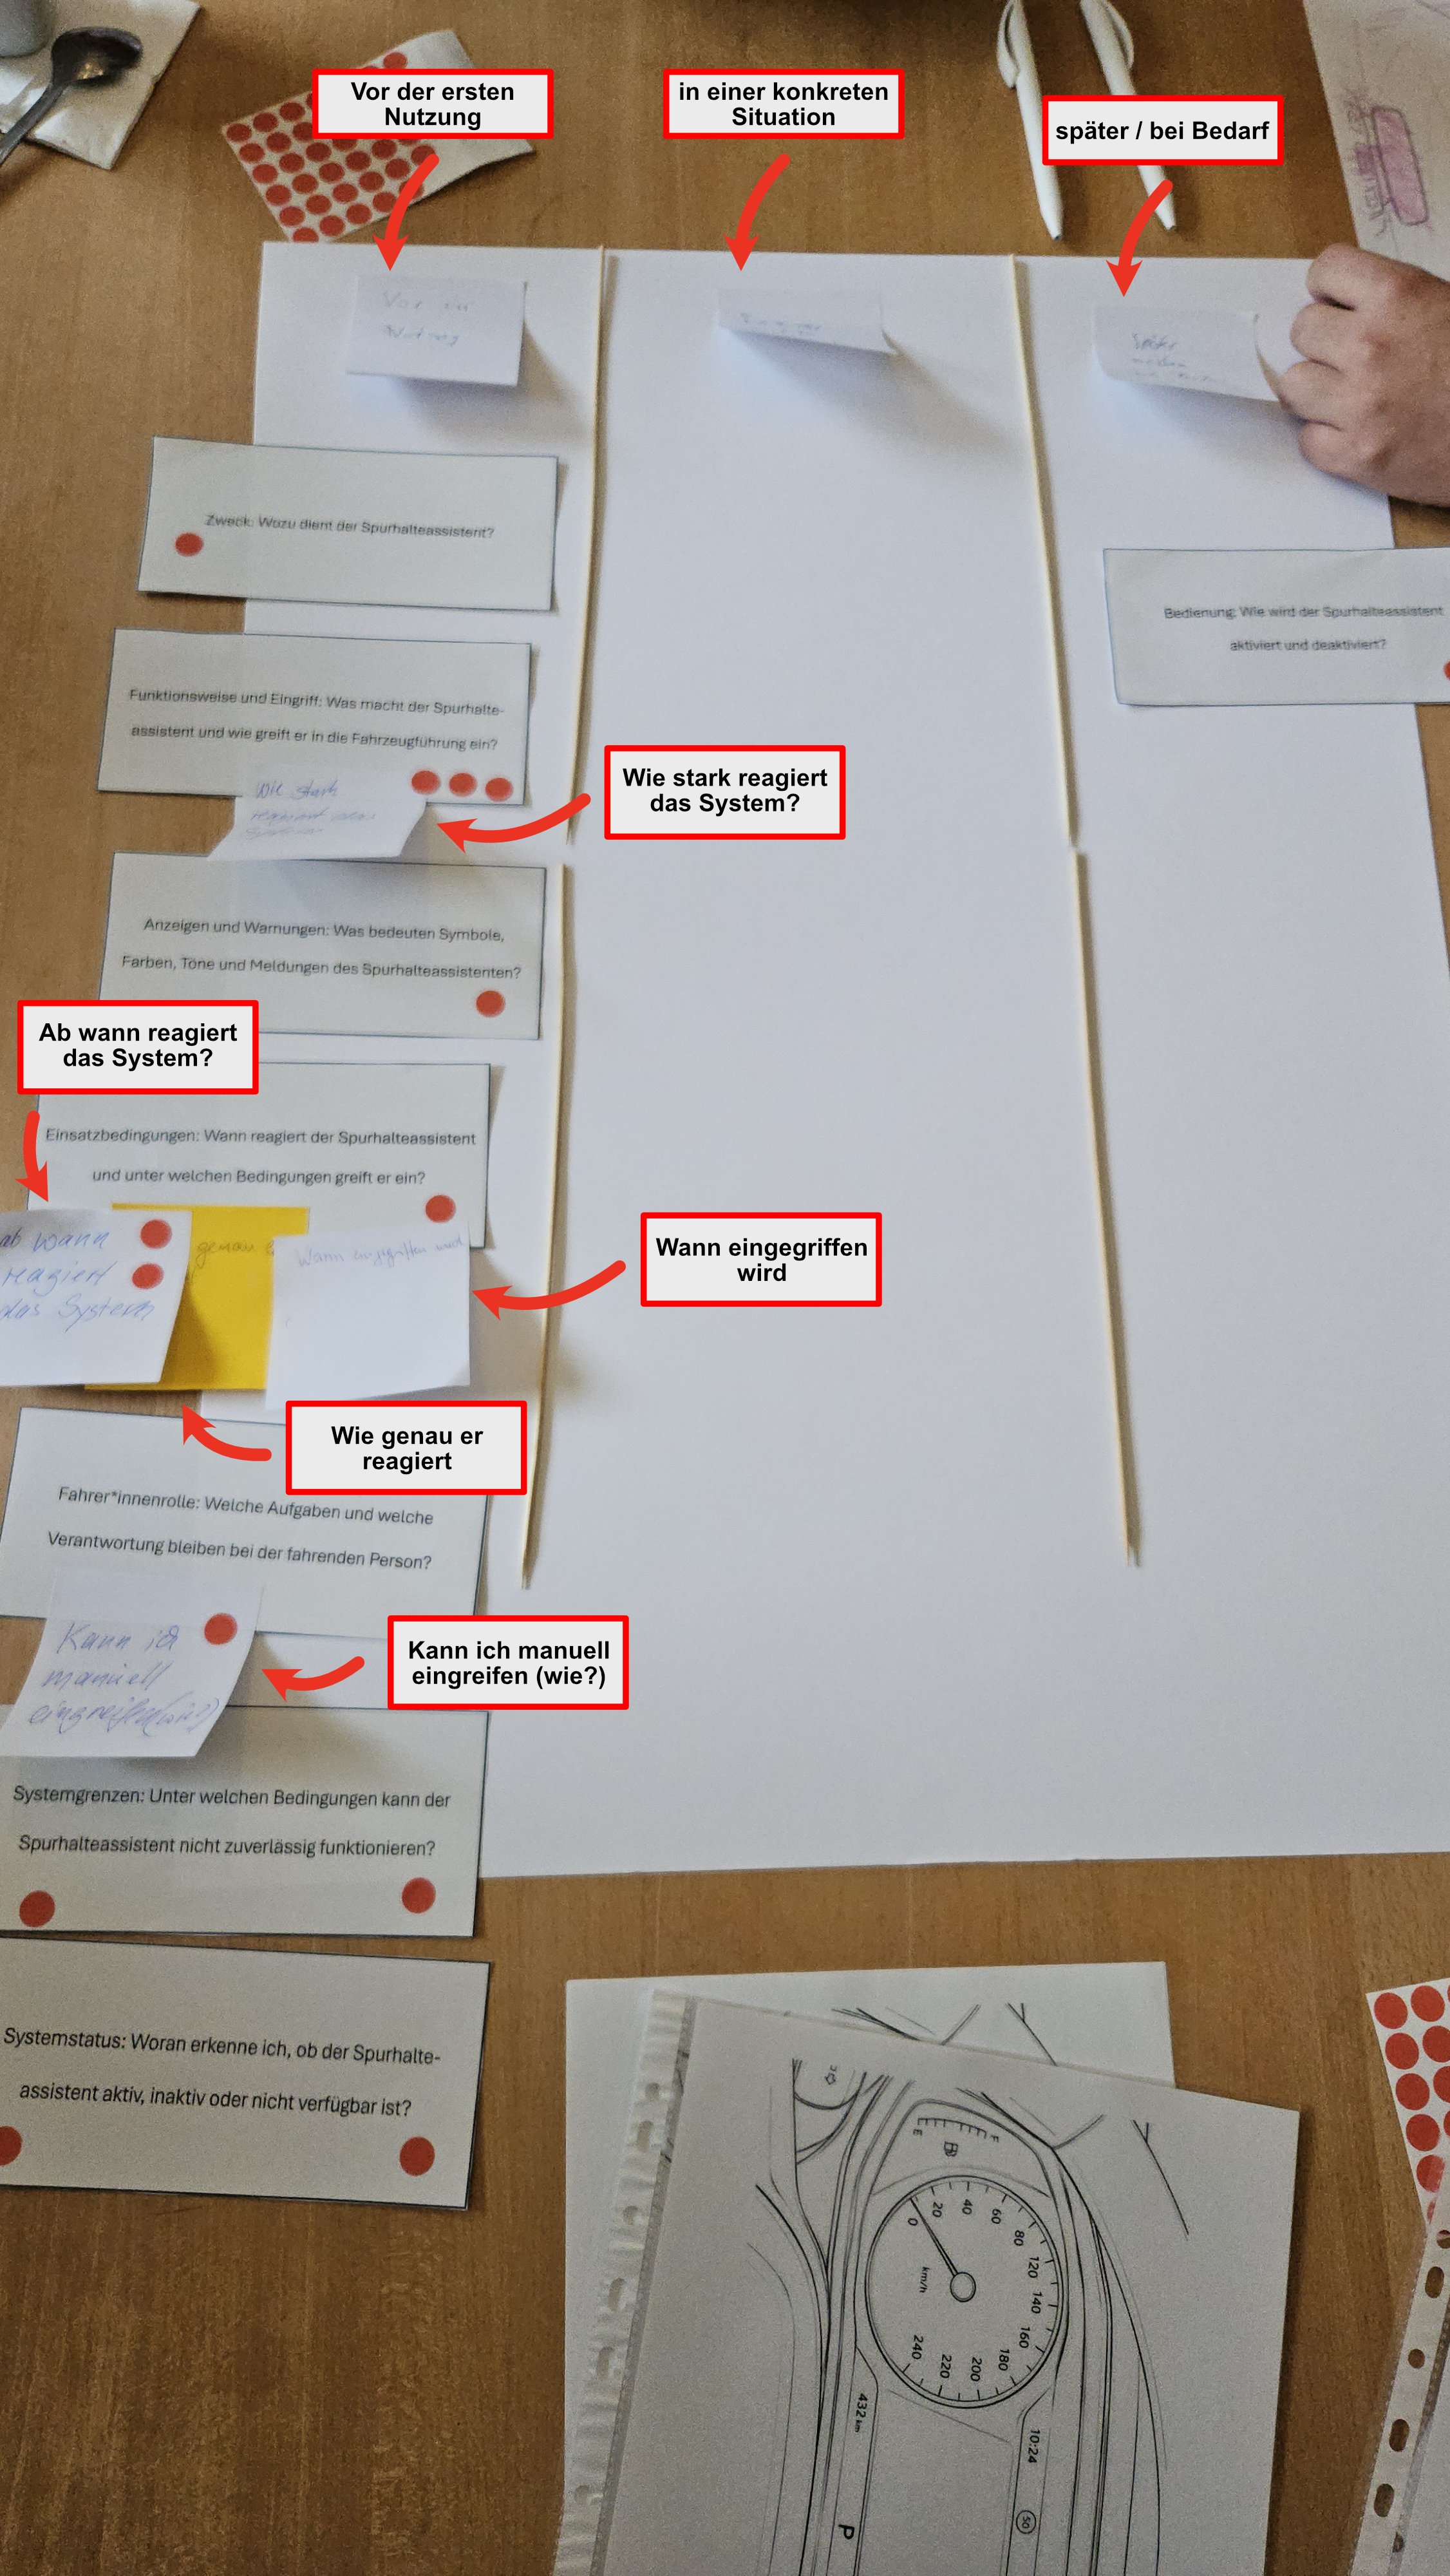
\includegraphics[width=0.65\textwidth]{images/results/Workshop_2/Ergebnisse_Choose_3.png}
    \caption{Ergebnisse der Choose-Phase des zweiten Workshops}
    \label{fig:W2_Choose_3}
    \medskip
    {\footnotesize Quelle: Eigene Fotografie.}
\end{figure}

Auch hier zeigt sich ein Muster, welches bereits im ersten Workshop deutlich wurde. Fast alle Themenkarten und Post-its werden in die Spalte einsortiert, welche eine Information vor der ersten Nutzung vorsehen. Die Aktivierung und Deaktivierung könne laut den Teilnehmer*innen jedoch später/bei Bedarf vermittelt werden. Auf Nachfrage der Moderation wurde dies damit begründet, dass erwartet wurde, dies sei die meiste Zeit nicht erforderlich.

\clearpage

Abbildung \ref{fig:W2_Commit} zeigt die abschließende Gegenüberstellung der Gestaltungsentwürfe zu den beiden Szenarien.

\begin{figure}[H]
    \centering
    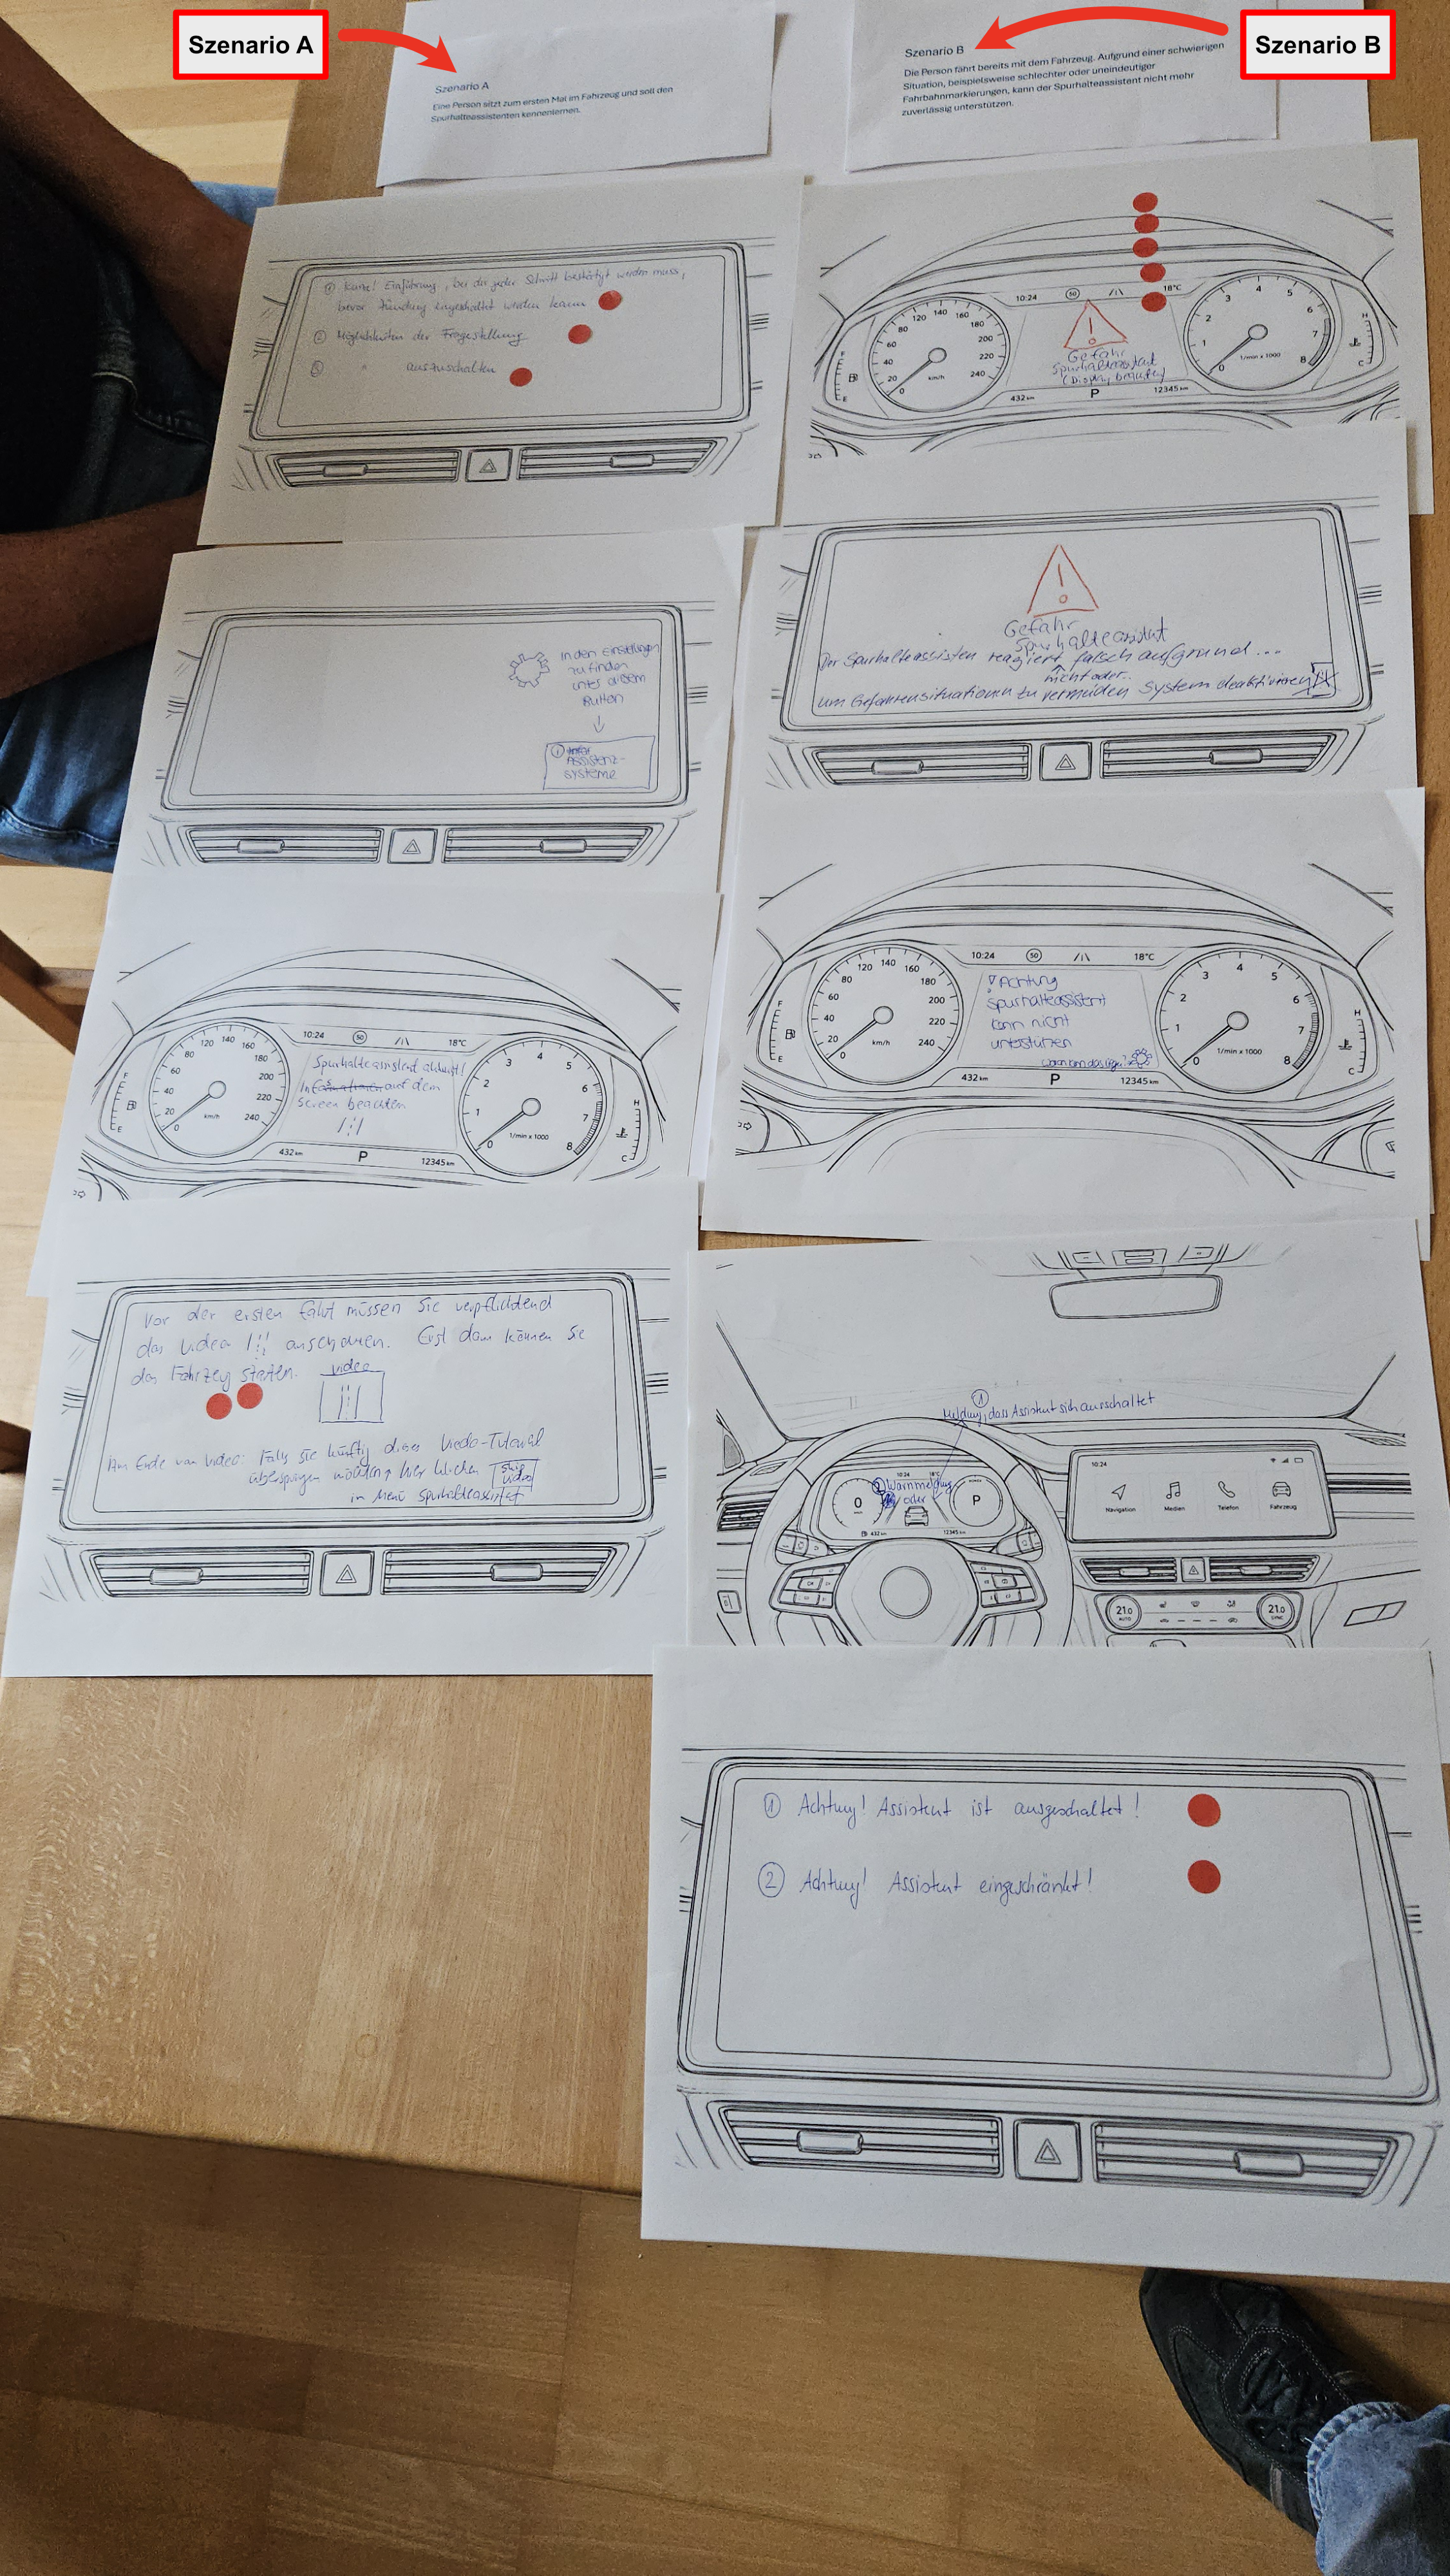
\includegraphics[width=0.65\textwidth]{images/results/Workshop_2/Ergebnisse_Commit.png}
    \caption{Ergebnisse der Commit-Phase des zweiten Workshops}
    \label{fig:W2_Commit}
    \medskip
    {\footnotesize Quelle: Eigene Fotografie.}
\end{figure}

Es zeigt sich, dass im Gegensatz zum ersten Workshop die genutzten Screens nahezu gleich zwischen beiden Szenarien verteilt sind. Allerdings sind die Klebepunkte und damit die Anzahl besonders hervorzuhebender Gestaltungselemente nicht gleichverteilt zwischen den den einzelnen Entwürfen. Stattdessen konzentrieren sie sich auf je zwei Gestaltungsentwürfe pro Szenario. Eine detaillierte Darstellung der Gestaltungsentwürfe findet sich analog zum ersten Workshop in Anhang \ref{sec:gestaltungslösungen_w2}.

\subsection{Design Features}
\label{subsec:Ergebnisse_Design_Features}

\section{Demonstration}
\label{Ergebnisse_Phase_vier}

\section{Evaluation}
\label{Ergebnisse_Phase_fünf}